\documentclass[12pt,oneside]{uhthesis}
\usepackage{subfigure}
\usepackage[ruled,lined,linesnumbered,titlenumbered,algochapter,spanish,onelanguage]{algorithm2e}
\usepackage{amsmath}
\usepackage{amssymb}
\usepackage{amsbsy}
\usepackage{caption,booktabs}
\captionsetup{ justification = centering }
%\usepackage{mathpazo}
\usepackage{float}
\setlength{\marginparwidth}{2cm}
\usepackage{todonotes}
\usepackage{listings}
\usepackage{xcolor}
\usepackage{multicol}
\usepackage{graphicx}
\floatstyle{plaintop}
\restylefloat{table}
\addbibresource{Bibliography.bib}
% \setlength{\parskip}{\baselineskip}%
\renewcommand{\tablename}{Tabla}
\renewcommand{\listalgorithmcfname}{Índice de Algoritmos}
%\dontprintsemicolon
\SetAlgoNoEnd

\definecolor{codegreen}{rgb}{0,0.6,0}
\definecolor{codegray}{rgb}{0.5,0.5,0.5}
\definecolor{codepurple}{rgb}{0.58,0,0.82}
\definecolor{backcolour}{rgb}{0.95,0.95,0.92}

\lstdefinestyle{mystyle}{
    backgroundcolor=\color{backcolour},   
    commentstyle=\color{codegreen},
    keywordstyle=\color{purple},
    numberstyle=\tiny\color{codegray},
    stringstyle=\color{codepurple},
    basicstyle=\ttfamily\footnotesize,
    breakatwhitespace=false,         
    breaklines=true,                 
    captionpos=b,                    
    keepspaces=true,                 
    numbers=left,                    
    numbersep=5pt,                  
    showspaces=false,                
    showstringspaces=false,
    showtabs=false,                  
    tabsize=4
}

\lstset{style=mystyle}

\title{Aprendizaje automático orientado a la clasificación de cáncer de piel. Un enfoque basado en EfficientNetB1}
\author{\\\vspace{0.25cm}Deborah Famadas Rodríguez}
\advisor{\\\vspace{0.25cm}Dr. Reinaldo Rodríguez Ramos, Universidad de la Habana\\\vspace{0.2cm}Dr. Yudivian Almeida, Universidad de la Habana}
\degree{Licenciado en Ciencia de la Computación}
\faculty{Facultad de Matemática y Computación}
\date{Fecha\\\vspace{0.25cm}\href{https://github.com/deborahfam/Thesis}{github.com/deborahfam/Thesis}}
\logo{Graphics/uhlogo}
\makenomenclature

\renewcommand{\vec}[1]{\boldsymbol{#1}}
\newcommand{\diff}[1]{\ensuremath{\mathrm{d}#1}}
\newcommand{\me}[1]{\mathrm{e}^{#1}}
\newcommand{\pf}{\mathfrak{p}}
\newcommand{\qf}{\mathfrak{q}}
%\newcommand{\kf}{\mathfrak{k}}
\newcommand{\kt}{\mathtt{k}}
\newcommand{\mf}{\mathfrak{m}}
\newcommand{\hf}{\mathfrak{h}}
\newcommand{\fac}{\mathrm{fac}}
\newcommand{\maxx}[1]{\max\left\{ #1 \right\} }
\newcommand{\minn}[1]{\min\left\{ #1 \right\} }
\newcommand{\lldpcf}{1.25}
\newcommand{\nnorm}[1]{\left\lvert #1 \right\rvert }
\renewcommand{\lstlistingname}{Ejemplo de código}
\renewcommand{\lstlistlistingname}{Ejemplos de código}

\begin{document}

\frontmatter
\maketitle

\begin{dedication}
    Dedicación
\end{dedication}
\begin{acknowledgements}
    De esta forma concluyen 5 años de duro y constante trabajo y aprendizaje que no hubieran sido posible sin cada una de esas personas que estuvieron siempre apoyándome en cada paso que daba, que nunca me dejaron rendirme y que si hoy estoy donde estoy, es gracias a ellos. Esta sección es para agradecerles.

    Bien saben mis padres que cuando pequeña no me despegaba un segundo de la computadora. Ese ímpetu por querer aprender cada vez más lo heredé de ellos. Por eso cuando tomé la decisión de coger una de las carreras más desafiantes en el mundo de la ciencia, no dudaron ni por un segundo en darme su apoyo incondicional. No fue fácil la trayectoria, viniendo de una provincia no necesariamente céntrica, teniendo que estar becada en el 'Bahía', pasar noches sin dormir y alejada de la familia, cada día seguía recibiendo ese mensaje de mi mamá: 'Cuqui, cómo va todo?' que me sacaba del estrés momentáneo y volvía a experimentar la tranquilidad. A mi mamá, que siempre luchó por mí, incluso cuando ni me lo merecía, incluso ni cuando las fuerzas le daban, que me ha hecho la mujer que soy y la que seré, le regalo esto que hoy construí y mucho más.

    De las abuelas se dice que son las que consienten a los nietos. Yo fui la primera de cuatro, su ' negrita bonita' (ni me pregunten por qué porque ni sé) y la más consentida. A mi 'Aya' le dedico esto. Por siempre decirme ' Pero tú eres inteligente, eso tú lo apruebas' lo mismo si le hablaba de Análisis matemático de 2 variables a si le hablaba de ' Educación física'. Ella fue la primera que vio en mi, lo que nadie, siempre sonriente, una sonrisa con algunas ventanas, pero con dirección al alma.
    
    Esta tesis tiene un halo mágico, y es que un angelito me ha estado velando todo el tiempo. 'Eo', nombre que mi subconsciente de pequeña le asignó a mi abuelo, fue y será parte de mi siempre. Nunca seré capaz de olvidar su risa 'kkkk' mientras me jalaba las orejas y me decía 'Ere una caballaaaa'. Él también se merece todo.

    A mi padre, que sabe amar a su forma única. El primero que me sentó delante de una computadora, que me cargaba a caballito y que al día de hoy sigue luchando por que yo salga adelante. A mis tíos, tías, primas, etc, con especial mención a mi tío 'Rene' que fue como un segundo padre para mí, y siempre estuvo cuando lo necesitábamos.

    Y continuando el tema de los agradecimientos familiares. Sería incorrecto de mí decir 'Le quiero agradecer a mis amigos', cuando son familia practicamente.

    Alguna vez se han fijado que somos muy poco agradecidos con el dedo pequeño del pie. Ese dedo que te ayuda a identificar obstáculos, incluso si tus ojos no pueden verlos (sobre todo si tus ojos no pueden verlos). Que te da estabilidad y soporte, que es gordito y aunque tiene 4 dedos más a los lados sigue siendo diferente. Yo tengo una persona así en mi vida, el 'Pocho' o como la gente lo llama 'Jean Pierre'. Es inconcluso de mi parte dedicarte un texto que no se empape en las lágrimas que derramaré si lo escribo, dado que solo tú y yo sabemos que significas. Te agradezco por tantas noches, tantas mañanas y tantas tardes, que no solo fuiste y eres amigo, mentor, el contacto más contactado y más importante de mi whatsapp, fuiste y eres TODO. Este mérito es completamente tuyo, esto y la libreta de discreta que tengo en la casa que a ver cuándo te la devuelvo jjj.
    
    A mi otra familia, Omar y Andy, que me apadrinaron desde primer año, que me han visto crecer y yo a ellos, que me dieron el primer cocotazo de la carrera y que hacen muchas veces mejor mis días. A Erick, a mi pepe grillo, tu forma de ser, por tu frialdad y a la vez tu cálido concepto de amistad, esto tampoco hubiera sido posible sin tí, y sin tus tacos que a ver cuando los vuelvo a probar. A David, porque no me lo perdonaría nunca si no te dedico unas líneas, contigo también fueron noches, incansables e incesantes de puro estrés al recibir por cuarta vez de mí la frase 'Ay que no te entiendo' y tú, tan calmado y confiado como siempre volver a la carga, siempre creyéndome capaz, sino como un hombre tan ocupado como tú hubiera dedicado tanto a una causa perdida jjj. A tí que fue muy importante ese abrazo luego de esa prueba de EDA, para tí también va esto.

    Comenta la gente que uno no se debe enamorar de sus mejores amigos, que rompe la amistad y que luego terminas arrepintiéndote. Pero una no puede cohibirse ante lo inevitable. Si bien besaste tú primero, no podría estar más agradecida al respecto. Y es que no hay otra voz más dulce que pueda calmar mi tormenta. Ay gaby, que más podría decirte que no haya dicho ya, que siempre estuviste ahí, a pesar que casa de lía te daba alergia, a pesar que solo tenías una muda de ropa, a pesar de todo, ibas, y solo el hecho de tenerte ahí era suficiente, es suficiente. Esto tampoco hubiera sido posible sin tí, y aunque lo dudes intensamente, te lo digo de corazón.

    Y quiero agradecer a todos, a mis tutores y mis profesores por llevarme a ser la profesional que soy hoy en día, al Dr. Jose Ignacio por sus consideraciones y consejos sobre la tesis que fueron de gran ayuda. A mis amigos del pre, por decirme 'Si mija coge eso, si al final, loca ya estás', a los amigos de la carrera, a Lachi, Alejandra, Roxana, Ana y Toni por sacarme de mi algarabía y disfrutar conmigo en las fiestas, por reírse de mis boberías en las conferencias y por siempre estar igual de estresados que yo con los exámenes. A mis suegros, que tan solo 10 meses en mi vida, mira que si han causado hueco sentimental. En fin, a todos aquellos que me ayudaron a lograr esto que hoy consigo.


\end{acknowledgements}
\begin{opinion}

El trabajo “Aprendizaje automático orientado a la clasificación de cáncer de piel: un enfoque basado en EfficientNetB1” presentado por la estudiante Deborah Famadas Rodríguez constituye un resultado notable en el campo de la biomedicina, bioinformática. En este trabajo de diploma se presenta una metodología para la clasificación automática del cáncer de piel mediante el uso de técnicas de aprendizaje profundo. La solución propuesta se basa en el uso de los pesos obtenidos de una red neuronal convolucional pre-entrenada, EfficientNetB1. Este proceso se beneficia del aprendizaje de grandes conjuntos de datos y experiencias previas para mejorar el reconocimiento de patrones en imágenes dermatológicas ya adquirido por la red convolucional. Luego se hace uso de un algoritmo propio de learning rate para ajustar el aprendizaje del modelo. 

Para la implementación de este marco de trabajo, el diplomante debió asimilar un volumen considerable de información, de disimiles campos, entre ellos el referente al aprendizaje profundo establecido como una importante subdisciplina dentro del aprendizaje automático, especialmente en áreas relacionadas con la percepción visual humana. Esta metodología procesa datos a través de múltiples capas que incluyen estructuras complejas y transformaciones no lineales. Actualmente ha logrado avances significativos en áreas como la visión artificial, el reconocimiento de voz, el procesamiento del lenguaje natural, el reconocimiento de audio y la bioinformática. El aprendizaje profundo se ha reconocido como uno de los diez avances tecnológicos más significativos, dadas sus amplias aplicaciones potenciales en el análisis de datos. El enfoque del aprendizaje profundo abstrae los datos en distintos niveles, lo que permite su aplicación en tareas complejas como la detección de objetos y la clasificación. Su capacidad para reemplazar la extracción manual de características por algoritmos eficientes de aprendizaje ya sea no supervisada o semi-supervisada, ha revolucionado múltiples áreas. Esta revolución incluye el campo de la atención médica, donde la gestión y análisis de un volumen abrumador de datos médicos es un desafío crucial.

El trabajo escrito presenta una estructura clara y organizada que permite fácil comprensión de los contenidos incluidos. Además de presentar los resultados obtenidos en su trabajo, el diplomante presenta elementos técnicos acerca de aprendizaje automático, otros elementos referentes a la programación como un grupo de técnicas y algoritmos tanto de las ramas de inteligencia artificial como del campo de la optimización, los cuales utiliza en el desarrollo de su trabajo, lo cual hacen del documento escrito un buen material de referencia para los futuros trabajos relacionados con el tema.

La diplomante ha trabajado con gran dedicación durante toda su trayectoria, lo caracterizan su constancia y dedicación al trabajo de investigación. Es una excelente estudiante con gran pasión por la investigación. Debe destacarse que tuvo que asimilar en un período muy corto todo un número de conceptos, definiciones, referentes a temas de la tesis, manejar una bibliografía compleja. Además, fue capaz de manera convincente y resuelta de enfrentar las dificultades con independencia, de manera creativa.

Por todo lo antes expuesto, le propongo al tribunal la evaluación del presente trabajo de excelente y que le sea concedida a Deborah Famadas Rodríguez el título de licenciado en Ciencia de la Computación. \\

\textbf{Tutores:} Dr. Reinaldo Rodríguez Ramos,
Dr Yudivian Almeida Cruz.

\end{opinion}
\begin{resumen}	
	El Machine Learning (Aprendizaje Automático) es una disciplina del campo de la Inteligencia Artificial que, a través de algoritmos, dota a los ordenadores de la capacidad de identificar patrones en datos masivos y elaborar predicciones \brackcite{Iberdrola2023MachineLearning}. Las Redes Neuronales Convolucionales (CNN), una especialización de esta disciplina, conocidas por su eficacia en el procesamiento de imágenes, son ideales para detectar características comunes en imágenes dermatológicas. 
	
	Este trabajo de diploma propone un algoritmo de machine learning, específicamente, una red neuronal, que permite extraer, a partir de un conjunto de imágenes de cáncer de piel, características para luego realizar una clasificación.
\end{resumen}

\begin{abstract}
	Machine Learning is a discipline in the field of Artificial Intelligence that, through algorithms, gives computers the ability to identify patterns in massive data and make predictions. Convolutional Neural Networks (CNN), a specialization of this discipline, known for their efficiency in image processing, are ideal for detecting common features in dermatological images. 
	
	This diploma work proposes a machine learning algorithm, specifically, a neural network, which allows extracting, from a set of skin cancer images, features to then perform a classification.
\end{abstract}
\tableofcontents
\listoffigures
\listoftables
% \listofalgorithms
% \lstlistoflistings

\mainmatter

\chapter*{Introducción}\label{chapter:introduction}
\addcontentsline{toc}{chapter}{Introducción}

Desde su surgimiento en 2006, el aprendizaje profundo se ha establecido como una importante subdisciplina dentro del aprendizaje automático, especialmente en áreas relacionadas con la percepción visual humana. Esta metodología procesa datos a través de múltiples capas que incluyen estructuras complejas y transformaciones no lineales \brackcite{lecun2015deep}. Actualmente ha logrado avances significativos en áreas como la visión artificial, el reconocimiento de voz, el procesamiento del lenguaje natural, el reconocimiento de audio y la bioinformática \brackcite{deng2014deep}. Desde 2013, el aprendizaje profundo se ha reconocido como uno de los diez avances tecnológicos más significativos, dadas sus amplias aplicaciones potenciales en el análisis de datos \brackcite{cai2020review}.

El enfoque del aprendizaje profundo abstrae los datos en distintos niveles, lo que permite su aplicación en tareas complejas como la detección de objetos y la clasificación. Su capacidad para reemplazar la extracción manual de características por algoritmos eficientes de aprendizaje, ya sea no supervisada o semi-supervisada, ha revolucionado múltiples áreas \brackcite{song2013hierarchical}. Esta revolución incluye el campo de la atención médica, donde la gestión y análisis de un volumen abrumador de datos médicos es un desafío crucial.

En el ámbito de la atención médica, especialmente en la dermatología, el aprendizaje profundo ha mostrado un potencial extraordinario. La dermatología, que se enfoca en el estudio y tratamiento de enfermedades de la piel, se enfrenta al desafío del cáncer de piel, el tipo de cáncer más frecuente a nivel mundial \brackcite{american_cancer_society_estadisticas_2023}. La detección precoz de este cáncer es vital \brackcite{american_cancer_society_estadisticas_2023}, y aquí es donde el aprendizaje profundo, con su habilidad para analizar y clasificar imágenes médicas con precisión, juega un rol transformador. La integración de estas tecnologías en la práctica dermatológica no solo mejora la precisión diagnóstica, sino que también promete revolucionar el tratamiento y manejo de diversas afecciones cutáneas \brackcite{fundacionpielsana_dermatologia}.

\section*{Motivación}

El uso de algoritmos de \textit{machine learning} (ML) para el diagnóstico del cáncer de piel puede resultar una herramienta valiosa. A diferencia de otros tipos de cáncer, el cáncer de piel se forma en la superficie de la piel y suele ser visible. Esto plantea una oportunidad única para la detección temprana y el tratamiento, lo cual es esencial, ya que la mayoría de los casos de cáncer de piel son tratables si se detectan a tiempo \brackcite{american_cancer_society_estadisticas_2023}.

Estos algoritmos pueden identificar patrones complejos con una precisión y consistencia mayor que los métodos de diagnóstico humano, reduciendo así la posibilidad de diagnósticos incorrectos debido a la interpretación subjetiva y variable de los expertos \brackcite{das2021machine}. Además, el ML puede procesar grandes volúmenes de datos rápidamente y su capacidad para aprender y adaptarse con el tiempo significa que la detección y clasificación del cáncer de piel puede mejorar continuamente \brackcite{das2021machine}.

Aunque ya existen algoritmos eficientes para la clasificación de melanomas, una forma de cáncer de piel, el desarrollo de un modelo capaz de clasificar varios tipos de cáncer de piel y generalizar entre ellos es todavía una Problemática abierta. Esto podría ampliar el alcance de las imágenes dermatológicas procesables, mejorando potencialmente la precisión en la detección y el tratamiento de distintas formas de cáncer de piel.


\section*{Antecedentes}

El desarrollo de las Redes Neuronales Convolucionales (CNN) ha sido fundamental para la identificación de características en imágenes médicas, una base sobre la cual se construye la motivación actual para aplicar ML en la dermatología. Su uso en medicina ha demostrado ser eficaz para capturar patrones específicos en datos de imágenes con alta precisión \brackcite{unal2023doc}.

Las universidades han desempeñado un papel crucial en la investigación y el desarrollo de tecnologías avanzadas en el campo de la medicina, especialmente en la detección y tratamiento del cáncer. Estos centros académicos no solo proporcionan una base sólida para la investigación teórica, sino que también fomentan la innovación práctica mediante el uso de tecnologías emergentes como el aprendizaje automático y la inteligencia artificial. En particular, nuestra universidad ha contribuido significativamente a este campo.

Un claro ejemplo de esta contribución es la tesis de Darien Viera Barredo titulada \textit{Autómata celular estocástico en redes complejas para el estudio de la invasión, migración y metástasis del cancer} \brackcite{automata_celular_thesis} proporciona un marco detallado sobre cómo se aborda el estudio del cáncer desde una perspectiva matemática y computacional avanzada. El modelo propuesto utiliza autómatas celulares estocásticos para simular el crecimiento avascular y vascular del tumor. En el se aborda la complejidad del ciclo vital tumoral, destacando la importancia de su comprensión tanto para la investigación del cáncer como para la salud pública. Tradicionalmente, la modelación matemática y computacional se ha centrado en las etapas tempranas del desarrollo tumoral, donde la mortalidad es baja. Sin embargo, este estudio se enfoca en las fases avanzadas, que son críticas para la vida del paciente.

Complementando esta línea de investigación, la tesis reciente de Claudia Olavarrieta Martínez \brackcite{ensemble_thesis} propone un \textit{ensemble} de redes neuronales para clasificar imágenes dermatoscópicas en cuatro categorías: melanoma, carcinoma basocelular, carcinoma espinocelular y otros utilizando la técnica de transferencia de conocimientos en redes como VGG16, ResNet50 y EfficientNet B0.



\section*{Problemática}

A pesar de los avances significativos en el campo del aprendizaje profundo y su aplicación en la detección y tratamiento del cáncer, como se evidencia en las investigaciones realizadas, aún persisten desafíos fundamentales. Uno de los principales retos es la necesidad de mejorar aún más la precisión y la eficiencia en el diagnóstico del cáncer de piel. Aunque los modelos actuales, han mostrado resultados prometedores, la diferenciación precisa entre diversas formas de cáncer de piel sigue siendo compleja, especialmente en etapas tempranas o en casos atípicos. Además, la mayoría de los modelos existentes se centran en la clasificación de melanomas, dejando de lado otras formas de cáncer de piel. Entonces \textbf{¿Es posible desarrollar un modelo avanzado de aprendizaje profundo que mejore significativamente la precisión y eficiencia en el diagnóstico de diversas formas de cáncer de piel, incluyendo tanto melanomas como otros tipos menos comunes, especialmente en etapas tempranas o en casos atípicos?} Se supone que, mediante la implementación de técnicas avanzadas de aprendizaje profundo y el análisis de un conjunto de datos más amplio y diversificado, se puede desarrollar un modelo que no solo clasifique con mayor precisión los melanomas, sino que también sea eficiente en la identificación de otras formas de cáncer de piel. Este modelo podría superar las limitaciones actuales y proporcionar un diagnóstico más preciso y temprano, lo que resultaría en un tratamiento más efectivo y una mejor tasa de supervivencia para los pacientes. Por lo tanto, el desarrollo de un modelo capaz de clasificar varios tipos de cáncer de piel y generalizar entre ellos es un objetivo crucial. Esto ampliaría el alcance de las imágenes dermatológicas procesables, mejorando potencialmente la precisión en la detección y el tratamiento.

\section*{Objetivos}

Este trabajo propone como objetivo fundamental el diseño y validación de un modelo predictivo basado en \textit{deep learning} para el diagnóstico del cáncer de piel mediante la clasificación de imágenes dermatológicas. El modelo se enfocará en clasificar imágenes, priorizando tanto la precisión de los resultados como la capacidad de generalización del modelo. \\


Entre los objetivos específicos del proyecto se encuentran:

\begin{enumerate}
    \item Estudiar el estado del arte sobre las técnicas empleadas en el diagnóstico de imágenes dermatológicas y su efectividad.
    \item Crear un modelo de \textit{deep learning} que dado un conjunto de imágenes de cáncer de piel clasifique el tipo al que pertenecen.
    \item Decidir, mediante una técnica de ML, la mejor distribución de datos para entrenamiento del modelo 
    \item Implementar mejoras potenciales al modelo y sus hiperparámetros para aumentar la precisión y generalización del mismo.
    \item Implementar técnicas de validación para evaluar la precisión del modelo.
\end{enumerate}

\section*{Estructura de la tesis}

El contenido de la tesis se organiza de la siguiente forma. En el capítulo 1 se exponen las principales alternativas presentes en la literatura que se han desarrollado para la clasificación de imágenes. En el capítulo 2 presenta el modelo propuesto para la implementación de un sistema de clasificación de imágenes de cáncer de piel. En los capítulos 3 y 4 se describe  los algoritmos y técnicas utilizadas, se describen los experimentos realizados y se exponen los resultados obtenidos y se analiza la efectividad de estos. Finalmente, se presentan las conclusiones de la tesis y las recomendaciones para investigaciones futuras.
\chapter{Estado del Arte}\label{chapter:state-of-the-art}

En las últimas décadas, los avances en potencia computacional han permitido un progreso significativo en el análisis automatizado de imágenes. Se ha pasado del análisis básico de imágenes digitales a sofisticados algoritmos capaces de identificar patrones sutiles en las imágenes de lesiones cutáneas. Los progresos en el reconocimiento de melanomas a partir de imágenes dermatológicas, han demostrado que los sistemas automatizados pueden lograr un diagnóstico comparable al de los expertos humanos \brackcite{DuHarpur2020}.   

\section{Teledermatología}

La teledermatología, una rama emergente de la telemedicina, ha revolucionizado el campo de la atención dermatológica. Impulsada por el auge de las tecnologías digitales a finales del siglo XX, esta modalidad se ha consolidado como una herramienta vital en el diagnóstico y manejo de afecciones cutáneas. Desde la década de 2000, la teledermatología ha permitido consultas dermatológicas remotas, ampliando significativamente el alcance de los servicios de salud \brackcite{romero2018practice}.

La investigación de Whited et al., en 2002, fue pionera en demostrar la efectividad de esta práctica \brackcite{whited2002teledermatology}. El estudio resaltó una reducción notable en los tiempos de respuesta, con una mediana de 5 días para consultas teledermatológicas, en contraste con los 28 días de los métodos tradicionales. Además, se enfatizó su utilidad en casos urgentes o semi-urgentes.

Paralelamente, la teledermatopatología ha mostrado su potencial, ofreciendo una fiabilidad comparable a la evaluación histológica tradicional \brackcite{romero2018practice}. Uno de los usos importantes de esta técnica fue detectar cáncer de piel. Un estudio, Piccolo et al., \brackcite{piccolo2002concordance} publicado en 2002, se centró en la concordancia entre los diagnósticos telepatológicos e histopatológicos convencionales, indicando contribuciones significativas en el campo de la teledermatopatología. Por término medio, el 78\% de los telediagnósticos fueron correctos (intervalo, 60\%-95\%), mientras que el 85\% de los diagnósticos convencionales fueron correctos (intervalo, 60\%-95\%). Se obtuvo una concordancia diagnóstica perfecta en 7 (35\%) de los 20 casos, y sólo se identificó una diferencia significativa en 1 caso.

Este avance en la teledermatología ha sentado las bases para la siguiente etapa en la medicina digital: el desarrollo de algoritmos computarizados que puedan detectar características en las imágenes, imitando el comportamiento humano, para luego a partir de estos obtener resultados.

\section{Técnicas tempranas de clasificación de imágenes} 

Cuando se trata de la clasificación de imágenes, es esencial considerar que nuestro sistema visual humano (SVH) primero recibe las ondas electromagnéticas que pertenecen al espectro visible y luego las interpreta en el cerebro. Sin embargo, en el campo de la visión artificial, cuando introducimos una imagen en un ordenador, lo que se interpreta es una matriz de números generalmente en el rango de [0,255] y con tres dimensiones en caso de que sea una imagen a color (RGB). Como resultado, se puede notar una gran brecha entre el significado semántico de la clase asociada a una imagen y los valores de píxeles que la componen, lo que hace que la tarea de clasificación sea compleja para sistemas artificiales \brackcite{unal2023doc}.

El reconocimiento de imágenes es una faceta de la inteligencia artificial que posibilita que los sistemas informáticos analicen e interpreten el contenido visual en imágenes. Esto se consigue detectando patrones y características distintivas que luego se emplean para clasificar y etiquetar objetos. Su propósito es automatizar el análisis visual, optimizando tiempo y recursos en diversas aplicaciones \brackcite{Qindel2023}. Esta tecnología se sustenta en algoritmos de aprendizaje automático, que entrenan a las máquinas para reconocer patrones visuales. Mediante el uso de bases de datos de imágenes etiquetadas para el entrenamiento, los algoritmos aprenden a identificar objetos y patrones. Una vez completado el entrenamiento, el modelo puede identificar automáticamente estos elementos en nuevas imágenes.

Desde finales del siglo XX, los ingenieros han dedicado esfuerzos significativos al desarrollo de técnicas y algoritmos para la categorización y reconocimiento de eventos a través de datos. Inicialmente, esto se centró en el procesamiento de texto para la clasificación automática de documentos, seguido por el tratamiento de sonidos e imágenes en diversos formatos. 

Un hito importante fue la publicación de un artículo sobre reconocimiento de patrones en 1974 en \textit{IEEE Transactions on Automatic Control} \brackcite{1100578}, evidenciando que ya en la década de $1970$ se estaban implementando estas técnicas en el reconocimiento de patrones. Los trabajos de este enfatizaron avances teóricos y experimentales significativos que impulsaron el progreso en el reconocimiento automático de patrones y el aprendizaje automático.

\subsection{Clasificación y reconocimiento de patrones en imágenes médicas}  

En el ámbito de la medicina, se ha observado que la mayoría de los sistemas artificiales de diagnóstico, en un punto, toman decisiones que están cada vez menos relacionadas con la apariencia física de la imagen tal como la vería un radiólogo. En su lugar, estos sistemas se basan en los detalles del patrón matemático de las características físicas individuales de la imagen, que son extraídas por un sistema de visión artificial o un radiólogo, para tomar su decisión final. Estos patrones matemáticos han sido objeto de estudio durante décadas por científicos que han utilizado diversos métodos analíticos, incluyendo las redes neuronales \brackcite{unal2023doc}.

Para abordar esta brecha entre la representación de la imagen y su significado, se han desarrollado varios tipos de algoritmos de clasificación. Algunos de estos algoritmos se basan en la detección de bordes, como el algoritmo de Canny \brackcite{datamount2023}. Sin embargo, estos algoritmos son robustos cuando se trata de identificar una clase específica, pero si se desea clasificar una clase diferente, es necesario crear un nuevo modelo desde cero \brackcite{rong2014improved}.

Esta serie de limitaciones restringieron su capacidad para abordar tareas complejas y desafiantes. La escasez de datos adecuados, la falta de recursos computacionales avanzados, arquitecturas simples, dificultades en el entrenamiento, generalización limitada, problemas de gradiente, falta de interpretabilidad y largos tiempos de entrenamiento fueron obstáculos clave en su desarrollo inicial.

Técnicas utilizadas en los inicios para la clasificación de patrones rompieron con algunas de las barreras de desarrollo: histograma de gradientes orientados (HOG) \brackcite{datasmarts_hog_scikit_image_2020}, Scale-Invariant Feature Transform (SIFT) \brackcite{lindeberg2012scale}, Binary Robust Independent Elementary Features (BRIEF) \brackcite{calonder2010brief}, Color Histograms \brackcite{pinecone_color_histograms}, entre otras. En la bibliografía se encuentran métodos de bajo nivel como son segmentación de la imagen por niveles grises, bordes o formas, entre otros y métodos de alto nivel como clasificadores basados en redes neuronales, máquinas de soporte vectorial (SVM), árbol de decisiones, entre otros \brackcite{leiva2019tecnicas}. 

Se destaca, además, que las tres técnicas más usadas en la clasificación automática de imágenes son árboles de decisiones, redes neuronales y máquinas de vectores de soporte siendo las redes neuronales una de las más utilizadas en campo del aprendizaje profundo \brackcite{leiva2019tecnicas}. 

\section{Introducción y desarrollo de \textit{machine learning} en el campo médico}

Las primeras aplicaciones de redes neuronales en imágenes médicas se orientaron hacia el análisis y clasificación de dichas imágenes para apoyar 
en diagnósticos y tratamientos. 

\subsection{Análisis de imágenes médicas}

El análisis de imágenes médicas mediante redes neuronales se ha enfocado en campos de la medicina como resonancia magnética, medicina nuclear y radiología, permitiendo la identificación y clasificación de patologías o condiciones específicas. Además, estas tecnologías han encontrado aplicaciones en áreas como la oftalmología, para el diagnóstico de enfermedades oculares a partir de imágenes de retina, y en la cardiología, para la evaluación de imágenes de ecocardiogramas \brackcite{unal2023doc}.

\begin{description}   
    \item Resonancia Magnética: En el contexto de la esclerosis múltiple, se han explorado soluciones de segmentación basadas en redes neuronales convolucionales (CNNs) para segmentaciones rápidas y fiables de lesiones y estructuras de materia gris en imágenes de resonancia magnética multimodal \brackcite{lee2022analysis}.
    
    \item Medicina Nuclear:  En este campo un estudio demuestra cómo el aprendizaje profundo puede restaurar la calidad de imagen diagnóstica y mantener la precisión de la cuantificación de SUV para exploraciones PET con un conteo reducido, lo que podría aumentar la seguridad y reducir el costo de las imágenes PET \brackcite{chaudhari2021low}.
    
    \item Radiología: En radiología, la aplicación de la inteligencia artificial en el análisis de imágenes de cáncer, con un enfoque en radiomía y representaciones derivadas del aprendizaje profundo, y su uso para el soporte de decisiones en la gestión del cáncer \brackcite{bera2022predicting}.
\end{description}

Esto muestra que el análisis de imágenes médicas a través de redes neuronales representa un avance significativo en diversas áreas de la medicina. Las aplicaciones van desde la identificación de patologías en resonancia magnética, medicina nuclear y radiología, hasta el diagnóstico de enfermedades oculares y la evaluación cardíaca. Estas tecnologías no solo mejoran la precisión en la detección y clasificación de condiciones específicas, sino que también optimizan la eficiencia de los procesos diagnósticos y terapéuticos, destacando el papel crucial de la inteligencia artificial en el futuro de la medicina. 

Teniendo en cuenta utilizando la inteligencia artificial se puede procesar grandes cantidades de datos, resulta una opción inteligente y acertada la recopilación de grandes volúmenes de datos (relacionados entre sí) para el procesamiento de los mismos con alguna herramienta de ML.

\section{Datasets de cáncer de piel}

En el campo de la dermatología, la generación de imágenes clínicas y dermatoscópicas es una práctica común para supervisar los cambios en las condiciones de la piel. Estas imágenes se han vuelto un recurso crucial para el avance de algoritmos de aprendizaje automático, especialmente en el desarrollo de Redes Neuronales Convolucionales (CNN). Los datasets son esenciales en ML porque proporcionan la base sobre la cual los algoritmos aprenden, se prueban, se comparan y evolucionan, permitiendo así la aplicación práctica y la innovación continua en este campo. Existen varios conjuntos de datos accesibles para la investigación en este ámbito.

Wu et al., recoge en su estudio un conjunto de los dataset de imágenes dermatologicas más utilizados en algoritmos de clasificación que se exponen a continuación:

\begin{itemize}
    \item El PH2 Dataset, compuesto por 200 imágenes dermoscópicas de tres tipos de enfermedades de la piel es ampliamente utilizado para probar algoritmos de diagnóstico de enfermedades de la piel, mostrando altas tasas de precisión en varios estudios \brackcite{wu2022skin}. 
    \item MED-NODE Dataset: Contiene 170 imágenes digitales de melanoma y nevus. Diversos métodos han mostrado resultados significativos de clasificación en este dataset \brackcite{wu2022skin}.
    \item HAM10000 Dataset: Recopilado por ISIC, incluye 10,015 imágenes dermoscópicas de siete enfermedades representativas de lesiones cutáneas pigmentadas. Se utiliza ampliamente en estudios de clasificación de cáncer de piel, superando a menudo el nivel de diagnóstico de los dermatólogos \brackcite{wu2022skin}.
    \item Derm7pt Dataset: Contiene aproximadamente 2,000 imágenes clínicas y de dermoscopia de enfermedades de la piel. Se ha utilizado para probar diversas redes multitarea y métodos de clasificación \brackcite{wu2022skin}.
    \item BCN20000 Dataset: Compuesto por 5,583 lesiones cutáneas y 19,424 imágenes dermoscópicas. Se emplea comúnmente en tareas de clasificación y segmentación de cáncer de piel \brackcite{wu2022skin}.
    \item ISIC Dataset: Con más de 13,000 imágenes dermoscópicas, se enfoca en la clasificación y segmentación del cáncer de piel, siendo utilizado en numerosos estudios y competiciones \brackcite{wu2022skin}.
\end{itemize}

Mientras que, entre otros autores Das et al., \brackcite{das2021machine} también menciona otros conjuntos de datos relevantes incluyen el Atlas Interactivo de Dermoscopia con 1000 ejemplos clínicos \brackcite{das2021machine}, la Biblioteca de Imágenes Dermofit con 1300 fotografías de alta resolución \brackcite{das2021machine}, el conjunto de datos de Asan \brackcite{das2021machine}, con 17,125 fotos clínicas, y el Hallym \brackcite{das2021machine}, con 125 fotos de casos de carcinoma basocelular. Además, los conjuntos de datos SD-198 y SD-260 \brackcite{das2021machine} ofrecen una amplia gama de imágenes clínicas de diversas enfermedades de la piel. Dermnet NZ y Derm7pt \brackcite{das2021machine} proporcionan colecciones extensas de fotografías clínicas, dermatoscópicas e histológicas, y The Cancer Genome Atlas \brackcite{das2021machine} presenta una de las mayores colecciones de diapositivas de lesiones cutáneas patológicas.

Entre todos estos conjuntos de datos, el HAM10000 se destaca por su amplia utilización en la investigación del cáncer de piel. Este conjunto de datos es particularmente valioso debido a su extensa colección de imágenes de lesiones de piel, que incluye una variedad de tipos de cáncer de piel. Su uso generalizado en la comunidad científica y su relevancia en estudios recientes lo convierten en el dataset ideal para el desarrollo de esta tesis. La riqueza y diversidad de las imágenes en HAM10000 proporcionan una base sólida para entrenar y evaluar algoritmos de \textit{machine learning}.

\section{Redes neuronales convolucionales en la medicina}   
El avance en la clasificación y detección de enfermedades de la piel, impulsado por los conjuntos de datos como HAM10000, ha preparado el camino para aplicaciones más sofisticadas en el análisis de imágenes médicas. En este escenario, las Redes Neuronales Convolucionales (CNN) emergen como una herramienta esencial, aprovechando la profundidad y variedad de los datos disponibles. Estas redes son especialmente eficaces en tareas de reconocimiento y clasificación visual, gracias a su capacidad para procesar y aprender de grandes volúmenes de imágenes.

Una red neuronal convolucional está formada por diferentes capas, entre ellas las principales son las capas convolucionales, las capas de max-pooling, y las capas completamente conectadas.La capa convolucional tiene como objetivo realizar la convolución a la imagen de entrada, para extraer sus características. Realizar una convolución a una imagen, consiste en filtrar dicha imagen utilizando una máscara o ventana. La máscara se va desplazando por toda la imagen, multiplicándose de forma matricial \brackcite{unal2023doc}.

En el campo de la medicina, estas facilitan la identificación de características relevantes en las imágenes médicas que pudieran ser indicativas de alguna condición médica particular. Se aprovechan de estructuras específicas de datos, como imágenes, para capturar patrones con mayor precisión, reducir la carga computacional y mejorar la generalización y la interpretabilidad. 

La evolución en la clasificación de lesiones cutáneas ha estado marcada por el uso innovador de redes neuronales convolucionales (CNNs). Una revisión sistemática en 2018 por Brinker et al., \brackcite{brinker2018skin} analizó 13 artículos que implementaban CNNs para esta tarea, destacando su alto rendimiento. Los enfoques más comunes involucraron la reutilización de CNNs ya entrenadas con grandes conjuntos de datos, optimizadas posteriormente para la clasificación específica de lesiones cutáneas. Esta metodología, aunque efectiva, enfrentó retos como la dificultad de comparar distintos métodos debido a la variabilidad en los conjuntos de datos.

Posteriormente, las técnicas de aprendizaje automático, y en particular los modelos de aprendizaje profundo, emergieron como herramientas poderosas para el análisis de imágenes médicas. Un proyecto clave fue \textit{A Deep Learning Approach to Skin Cancer Detection in Dermoscopy Images} \brackcite{ameri2020deep}, donde se utilizó un conjunto de 3400 imágenes dermatoscópicas del HAM10000, incluyendo lesiones melanoma y no melanoma. Se implementó una red neuronal convolucional profunda que procesaba imágenes directamente, identificando características valiosas sin necesidad de segmentación previa, lo cual representó un avance significativo en la simplificación y eficacia del proceso de clasificación.

En 2022, el estudio \textit{Skin lesion classification of dermoscopic images using machine learning and convolutional neural network} \brackcite{shetty2022skin}, publicado en Nature, utilizó un subconjunto del HAM10000 para clasificar lesiones cutáneas mediante aprendizaje automático y CNN. Este enfoque ofreció resultados prometedores en la distinción entre lesiones malignas y benignas, logrando una precisión del 95,18\% con el modelo CNN. La comparación con otros algoritmos de aprendizaje automático resaltó la superioridad de los modelos CNN en términos de precisión.

Tajerian , \brackcite{tajerian2023design} presentó un enfoque metodológico para mejorar el diagnóstico de la lesiones cutáneas pigmentadas utilizando imágenes dermatoscópicas del conjunto de datos HAM10000. Este conjunto de datos se utilizó para analizar lesiones cutáneas pigmentadas. El modelo obtiene los mejores resultados en la detección de lesiones de nevos melanocíticos,con una puntuación F1 de 0,93.

Adegun et al., \brackcite{adegun2021deep} recoge un conjunto de artículos que contribuyeron al desarrollo de algoritmos además de los anteriormente mencionados. Las referencias a los siguientes artículos están recogidas en el mismo \brackcite{adegun2021deep}:

\begin{enumerate}
    \item Majtner et al., usaron técnicas de CNN para la extracción de características y preprocesamiento, utilizando el conjunto de datos ISIC con 900 muestras de entrenamiento y 379 de prueba, clasificadas en benignas y malignas \brackcite{adegun2021deep}. 

    \item Vipin et al.,  implementaron un sistema de dos etapas, segmentación y clasificación, utilizando un conjunto de datos ISIC de 13,000 imágenes, reducido a 7,353 tras eliminar imágenes no utilizables \brackcite{adegun2021deep}. 

    \item Nasr-Esfahani et al.,  desarrollaron su propia CNN para preprocesar, extraer características y clasificar imágenes, con un conjunto de 170 imágenes no dermatoscópicas del UMCG, aumentado a 6,120 imágenes \brackcite{adegun2021deep}. 

    \item Attia et al., usaron una CNN completamente conectada con arquitecturas de autoencoder-decoder, alcanzando una precisión del 98\% y una especificidad del 94\% \brackcite{adegun2021deep}. 

    \item Mukherjee et al., desarrollaron una arquitectura CNN para la detección de lesiones malignas, logrando precisiones de 90.14\% y 90.58\% en los conjuntos de datos MEDNODE y Dermofit \brackcite{adegun2021deep}. 

    \item Sanketh et al., propusieron una CNN para la detección temprana de cáncer de piel, obteniendo un resultado óptimo del 98\% \brackcite{adegun2021deep}. 

    \item Rahi et al., propusieron un modelo CNN con varias capas convolucionales y de agrupación máxima, logrando una precisión del 84.76\% y una especificidad del 78.81\% \brackcite{adegun2021deep}. 

    \item Gulati et al., emplearon redes preentrenadas como AlexNet y VGG16, obteniendo mejores resultados con VGG16 en modo de aprendizaje transferido \brackcite{adegun2021deep}.
    \item Daghrir et al.,combinaron una CNN con técnicas de aprendizaje automático clásicas, alcanzando una precisión individual del 85.5\% con CNN \brackcite{adegun2021deep}. 

    \item Acosta et al., incorporaron técnicas de CNN basadas en máscaras y regiones con una estructura ResNet152 preentrenada, logrando una precisión del 90.4\% y una especificidad del 92.5\% \brackcite{adegun2021deep}.

\end{enumerate}

El avance en la detección de cáncer mediante el uso de la inteligencia artificial (IA) y el aprendizaje automático (ML) ha sido significativo en las últimas décadas. El mismo ha demostrado un rendimiento excepcional en tareas de reconocimiento de imágenes, que es fundamental en la detección del cáncer de piel. Se llevó a cabo una revisión exhaustiva para evaluar el impacto de las técnicas de aprendizaje profundo en la detección precoz, en la que se analizaron diversos resultados de investigación y se presentaron mediante herramientas, gráficos, tablas y marcos para comprender mejor las técnicas predominantes en este campo \brackcite{dildar2021skin}.

\section {Trabajos basados en EfficientNet}

Uno de los modelos de redes convolucionales que ha tenido relevacia es EfficientNet. Este es una familia de modelos de red neuronal convolucional diseñada para la eficiencia, que significa que pueden lograr una mayor precisión con menos parámetros y computación. Es un novedoso método de escalado de modelos que utiliza un coeficiente compuesto sencillo pero muy eficaz para escalar las CNN de forma más estructurada \brackcite{tan2019efficientnet}.

Un estudio innovador relacionado con EfficientNet es el de Ali et al., \brackcite{ali2022multiclass}. Este desarrolló una cadena de procesamiento de imágenes previo al entrenamiento, que incluía la eliminación de cabellos en las imágenes, el aumento de datos y el redimensionamiento de las imágenes para cumplir con los requisitos de cada modelo de CNN. Utilizando transferencia de aprendizaje con pesos pre-entrenados de ImageNet y ajuste fino de las redes, se entrenaron variantes de EfficientNet (B0-B7) en el conjunto de datos HAM10000. El modelo más exitoso, EfficientNet B4, alcanzó una puntuación F1 y una precisión Top-1 del 87\% y 87.91\%, respectivamente, destacando que una complejidad intermedia del modelo puede ser óptima para este tipo de tareas. El modelo en cuestión relacionado con nuestro enfoque (EfficientNetB1) obtuvo una precisión del 86.5\% y una precisión Top-1 del 86.5\%.

Por otro lado Papiththira et al. \brackcite{papiththira2021melanoma} se centró específicamente en la detección de melanoma utilizando un enfoque basado en transferencia de aprendizaje profundo sin necesidad de preprocesamiento de imágenes. Este método se apoyó en el modelo EfficientNet pre-entrenado, complementado con un módulo de atención de canales para resaltar características específicas del melanoma en la clasificación. Evaluado en los conjuntos de datos UMGC y HAM10000, que incluyen imágenes clínicas y dermoscópicas, el enfoque propuesto superó los métodos del estado del arte con una precisión de clasificación del 84.12\% y 96.32\%, respectivamente.

\section{Conclusión del estado del arte}

Es notable un progreso en el análisis automatizado de imágenes, especialmente en el ámbito médico. Este avance ha sido impulsado significativamente por el desarrollo en la potencia computacional y la inteligencia artificial, lo que ha facilitado un diagnóstico más preciso y rápido de enfermedades. Paralelamente, el campo de la dermatología ha experimentado una revolución con la introducción de la teledermatología y teledermatopatología, mejorando la accesibilidad a servicios especializados y permitiendo diagnósticos rápidos y precisos a distancia, lo que es esencial para el tratamiento oportuno de enfermedades cutáneas.

Además, se ha destacado la importancia de los conjuntos de datos en el aprendizaje automático, como el HAM10000, que han sido cruciales en el desarrollo de algoritmos en dermatología. Estos datasets proporcionan una base diversa y rica para el entrenamiento y evaluación de modelos, contribuyendo a avances significativos en la clasificación y detección de enfermedades de la piel. En términos de técnicas de clasificación de imágenes, se ha observado una evolución desde métodos iniciales como el procesamiento de bordes hasta el uso de algoritmos avanzados de aprendizaje automático y profundo. Las redes neuronales, en particular, han mostrado ser herramientas excepcionales para el análisis de imágenes médicas, aumentando la precisión y eficiencia en la identificación de patologías.

El papel de las redes neuronales convolucionales (CNN) en medicina ha sido fundamental, especialmente en dermatología, donde han posibilitado avances significativos en la clasificación de lesiones cutáneas. Los modelos basados en CNN han alcanzado una precisión comparable a la de especialistas humanos, lo que sugiere un futuro prometedor para la inteligencia artificial en el diagnóstico y tratamiento de enfermedades.

Sin embargo, a pesar de estos avances, todavía persisten desafíos como la variabilidad en los conjuntos de datos y la necesidad de mejorar la generalización de los modelos. Estos retos ofrecen oportunidades para futuras investigaciones y desarrollos, en particular en la mejora de algoritmos y en la integración de nuevas tecnologías en la práctica médica.
\chapter{Propuesta de solución}\label{chapter:proposal}

Este capítulo introduce la propuesta desarrollada para enfrentar el reto de clasificar de manera automática el cáncer de piel, empleando técnicas de aprendizaje profundo. La solución se centra en la utilización de una red neuronal profunda pre-entrenada, combinada con un algoritmo propio para el ajuste de precisión.

En el núcleo de nuestra estrategia se encuentra el uso de una red neuronal convolucional pre-entrenada llamada \textit{EfficientNetB1}. Esta red, desarrollada a partir de extensos conjuntos de datos y experiencias previas, ofrece una base sólida y rica en características para nuestro modelo. Al aprovechar este pre-entrenamiento, se puede acelerar significativamente el proceso de aprendizaje del modelo, al tiempo que aumentamos su capacidad para generalizar y reconocer patrones complejos en las imágenes dermatoscópicas.

Para complementar el enfoque metodológico, se seleccionan un conjunto de herramientas tecnológicas avanzadas. Estas herramientas están diseñadas para optimizar el rendimiento del modelo, mejorar la precisión de la clasificación y garantizar una implementación efectiva. Entre ellas, destaca una capa de normalización, una capa densa, una de regularización, una de \textit{dropout} y una de salida (capa densa con activación \textit{softmax}). Estas técnicas le permiten al modelo afinar su capacidad de identificar con precisión las diferentes categorías de lesiones cutáneas.

Para la optimización del algoritmo además se llevaron a cabo una serie de experimentos de los que se detallan al final de este capítulo los 2 más relevantes. Estos experimentos se realizaron con el objetivo de encontrar la mejor configuración de datos para el modelo, que permita obtener la mayor precisión posible. Para esto se utilizaron dos técnicas de normalización de datos: division asimétrica con utilización de pesos por clases y estratificación de datos. Además, se generaron distintas distribuciones de datos para los diferentes acercamientos.

Con la intensión de evaluar la efectividad y precisión del modelo se hizo uso del conjunto de datos mencionado previamente: HAM1000. Este, con más de 10000 imágenes, representa una variedad de condiciones de la piel, lo que lo convierte en un recurso valioso para entrenar y evaluar algoritmos de detección de cáncer de piel. Para esto se importan, modelan y dividen los datos para asegurar un aprendizaje efectivo

La sección que sigue detalla la metodología empleada en la preparación y carga de los datos. Esta fase es esencial, ya que la calidad y el tratamiento de los datos tienen un impacto directo en la eficacia del modelo.

\begin{figure}[H]
   \begin{center}
   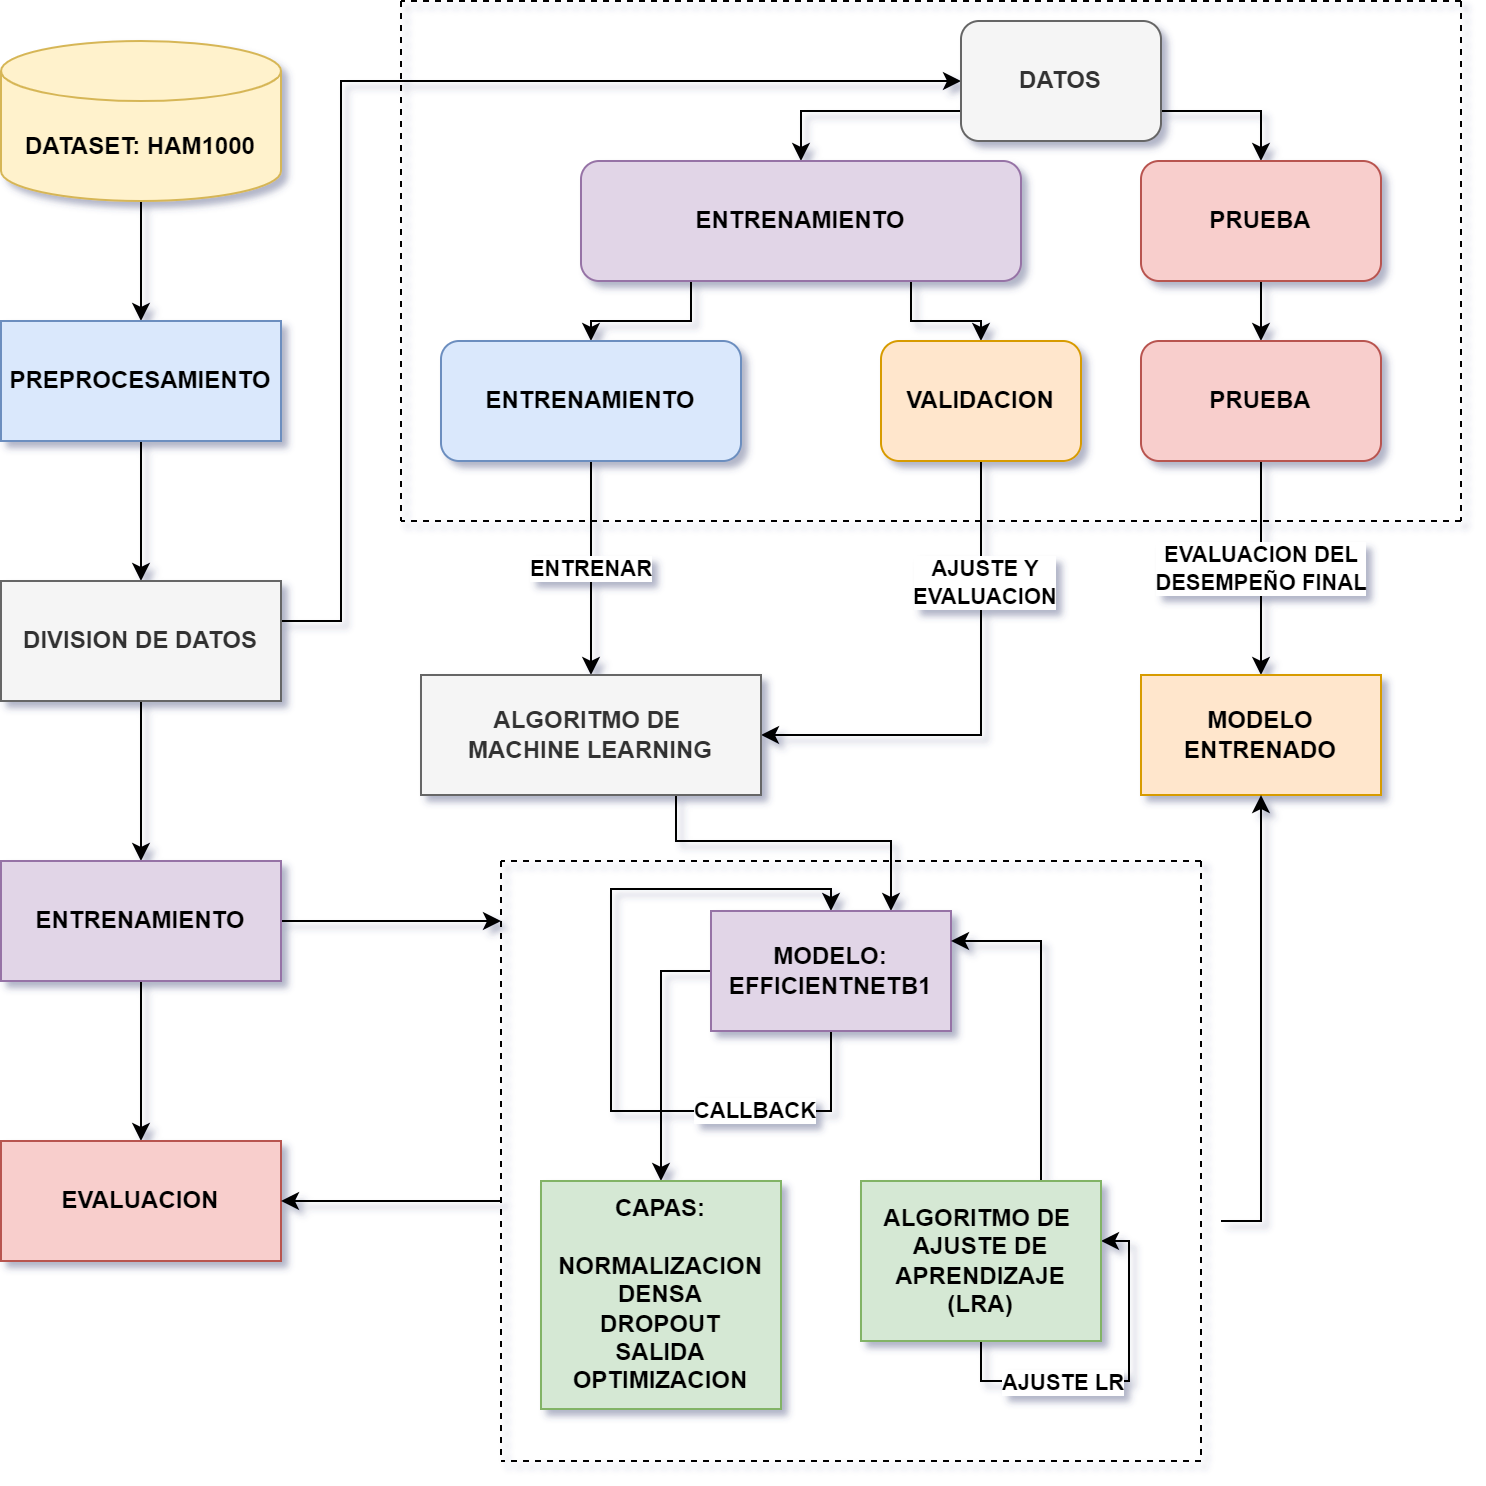
\includegraphics[width=1\textwidth]{./Graphics/model.png}
   \caption{Diagrama de flujo del proceso de entrenamiento  y validación del modelo.}
   \label{fig:model_structure}
   \end{center}
   \end{figure}

\section{Preparación y carga de datos}

En la presente sección, se describe cómo se seleccionó y procesó el conjunto HAM10000. Se detallan técnicas aplicadas para optimizar el rendimiento del algoritmo incluyendo el procesamiento de las imágenes y la conversión de los metadatos a un formato categórico adecuado para su análisis.

Posteriormente, se explica la modelación y división del conjunto de datos, utilizando herramientas como Pandas para estructurar los datos y dividirlos en conjuntos de entrenamiento, validación y prueba. Finalmente, se aborda el desafío del desequilibrio en la representación de las clases dentro del \textit{dataset}. Se detallan las estrategias implementadas para equilibrar el conjunto de datos, garantizando así que el modelo aprenda de manera efectiva a identificar una variedad de lesiones cutáneas sin sesgos hacia las condiciones más comunes.

\subsection{Dataset}

El conjunto de datos HAM10000, acrónimo de \textit{Human Against Machine with 10000 training images} (Humano Contra Máquina con 10000 imágenes de entrenamiento), se presenta como una solución al problema de la falta de diversidad y tamaño reducido en los conjuntos de datos disponibles para el diagnóstico automatizado de lesiones cutáneas pigmentadas. Este conjunto de datos es notable por su extenso alcance y diversidad, abarcando una amplia gama de lesiones cutáneas pigmentadas comunes \brackcite{tschandl2018ham10000}. 

\subsubsection*{HAM10000}

Las $10015$ imágenes dermatoscópicas del conjunto de datos HAM10000 se recopilaron a lo largo de 20 años desde dos ubicaciones diferentes: el Departamento de Dermatología de la Universidad Médica de Viena, Austria, y la práctica de cáncer de piel de Cliff Rosendahl en Queensland, Australia \brackcite{tschandl2018ham10000}. En comparación con otros conjuntos de datos, HAM10000 ofrece un conjunto más diverso y completo de imágenes dermatoscópicas para la investigación del aprendizaje automático. Las imágenes y los metadatos del HAM10000  tienen la siguiente distribución.

\begin{table}[H]
   \centering
   \small
   \begin{tabular}{lccc}
   \hline
   \textbf{Categoría Diagnóstica} & \textbf{Cantidad} & \textbf{Porcentaje} \\
   \hline
   Melanocytic nevi (NV) & 6705 & 66.95\%  \\
   Melanoma (MEL) & 1113 & 11.11\% \\
   Benign keratosis-like lesions (BKL) & 1099 & 10.97\% \\
   Basal cell carcinoma (BCC) & 514 & 5.13\% \\
   Actinic Keratosis and Intraepithelial Carcinoma (AKIEC) & 327                         & 3.27\%              \\
   Vascular lesions (VASC) & 142 & 1.42\%  \\
   Dermatofibroma  (DF) & 115 & 1.15\% \\
   \hline
   \end{tabular}
   \caption{Distribución de imágenes por categoría diagnóstica.}
   \label{tab:ham10000_distribution}
\end{table}   
   
Las imágenes almacenadas, originalmente como diapositivas, fueron digitalizadas usando un escáner \textit{Nikon Coolscan 5000 ED}. Posteriormente, se ajustaron manualmente para centrar las lesiones y se aplicaron correcciones al histograma para mejorar el contraste visual y la reproducción del color. Para separar eficientemente las imágenes dermatoscópicas de otros tipos de imágenes (como primeros planos y vistas generales), se utilizó un método automatizado que clasificaba más de 30,000 imágenes. Se empleó una arquitectura \textit{InceptionV3}, entrenada con un conjunto de imágenes etiquetadas manualmente, para categorizar las imágenes. Las imágenes mal clasificadas por este método fueron revisadas y corregidas manualmente.  Se realizó una revisión manual final para excluir imágenes con ciertos atributos no deseados, como contenido potencialmente identificable, imágenes fuera de enfoque o con artefactos perturbadores como prendas, y lesiones completamente no pigmentadas. Las imágenes restantes fueron revisadas para asegurar una reproducción de color y luminosidad adecuadas, aplicando correcciones manuales si era necesario \brackcite{tschandl2018ham10000}. 


Los datos utilizados como medio de aprendizaje para este proyecto son imágenes y metadatos. El dataset HAM10000 contiene imágenes y un archivo de metadatos que contienen información relacionada con cada imagen en formato \textit{one hot encoding} \brackcite{ohe}.

\subsection{Transformación de datos}

Los metadatos asociados a la clasificación, etiquetados con el método mencionado (\textit{one hot encoding}), fueron convertidos a un formato \textit{categórico} \brackcite{vitalflux_categorical_crossentropy} para su procesamiento. En este proceso a cada elemento se le asignó una etiqueta basada en las categoría de la lesion cutánea, como 'MEL' (Melanoma), 'NV' (Nevus Melanocítico), entre otras. Se elimina del \textit{dataframe}, además, cualquier columna innecesaria, dejando solo las etiquetas y nombres de imágenes relevantes. De tal forma que los datos quedan distribuidos por clase.

\begin{table}[H]
   \centering
   \begin{tabular}{lccc}
   \hline
   \textbf{Index} & \textbf{Imágenes} & \textbf{Etiqueta} \\
   \hline
      0 & $ISIC\_0024306.jpg$ & NV \\
      1 & $ISIC\_0024307.jpg$ & NV \\
      2 & $ISIC\_0024308.jpg$ & NV \\
      3 & $ISIC\_0024309.jpg$ & NV \\
      4 & $ISIC\_0024310.jpg$ & MEL \\
   \hline
   \end{tabular}
   \caption{Datos transformados a formato categórico.}
   \label{}
\end{table}   

\subsection{Modelación y división del conjunto de datos}

Los datos se modelan a partir de un \textit{dataframe} de Pandas \brackcite{pandas}. Estos son divididos en 3 conjuntos: Entrenamiento, Validación y Prueba, utilizando un enfoque simple de division de datos en porcentaje. Estas divisiones son necesarias para que el modelo pueda aprender y ser evaluado correctamente.

Inicialmente, el conjunto de datos, fue dividido en dos subconjuntos: \textit{train}, que se destinó para el entrenamiento, y \textit{dummy}, que fue utilizado como una combinación temporal para los conjuntos de validación y prueba. Luego el segundo conjunto fue separado en \textit{valid}, destinado a la validación y \textit{test}, utilizado para las pruebas.

\subsection{Generadores de datos y preprocesamiento}

Uno de los principales problemas del \textit{dataset}, como se puede observar en la tabla 2.1, es el desequilibrio en la representación de las clases, un problema habitual en los conjuntos de datos médicos en los que algunas enfermedades son más raras que otras. Para solucionar este problema, el conjunto de datos se equilibra limitando el número máximo de muestras por clase. Esto garantiza que el modelo no esté sesgado hacia las clases más comunes y pueda generalizar mejor entre varios tipos de lesiones cutáneas. 

La cantidad de muestras por clase se ajustó de manera selectiva. Incluso con estas transformaciones algunas clases seguían desbalanceadas, lo que llevó a la implementación de la técnica de \textit{class weighting} \brackcite{analyticsvidhya2020classweight}. Con este método se asignó pesos diferenciados a cada clase durante el entrenamiento del modelo, reforzando así la señal de aprendizaje para las clases menos representadas.

Además, a los conjuntos segmentados en entrenamiento, validación y prueba, se les aplicó \textit{data augmentation}. Esta técnica aplicó varias transformaciones a las imágenes, como rotación, desplazamiento y zoom, durante su carga, generando lotes de imágenes optimizados para el entrenamiento y evaluación del modelo \brackcite{augmentation}.

\section{Desarrollo del modelo y estrategias de optimización}\label{sec:method}
%-----------------------------------------------------------------------------------

Para abordar efectivamente el desafío de la detección de cáncer de piel, se seleccionó la arquitectura \textit{EfficientNetB1} \brackcite{efficientnet} como base del modelo. Esta red neuronal convolucional, parte de la familia EfficientNet, se caracteriza por su alta eficiencia y precisión. Utilizando un modelo pre-entrenado, se aprovecharon los pesos derivados de conjuntos de datos extensos, lo que facilitó la adaptación del modelo a nuestro conjunto de datos específico (HAM10000) \brackcite{tan2019efficientnet}.

\subsection{Diseño y entrenamiento del modelo}

El modelo \textit{EfficientNetB1} se carga pre-entrenado con pesos de \textit{ImageNet} \brackcite{Pinecone2021ImageNet}, una amplia base de datos de imágenes ampliamente utilizada para entrenamiento y \textit{benchmarking} en visión por computadora. Luego a este se le omitió la capa superior. Al omitir la capa superior del modelo, se permite la incorporación y personalización de capas adicionales que se mencionan más adelante en el capítulo. Además, la salida del modelo base se somete a una serie de transformaciones, incluyendo normalización por lotes, capas densas con regularizaciones, y técnicas de \textit{Dropout} para prevenir el sobre-ajuste, culminando en una capa de salida optimizada para la clasificación.

\subsubsection{Arquitectura del modelo EfficientNet}
   
La familia de arquitecturas EfficientNet \brackcite{tan2019efficientnet}, surgió con el objetivo de hallar un método adecuado para escalar las CNNs de manera que mejoraran tanto en precisión (i.e., rendimiento del modelo) como en eficiencia (es decir, en términos de parámetros del modelo y FLOPS). 

Inicialmente, el enfoque se centraba en aumentar la profundidad o el ancho de la red. Sin embargo, este método de escalado único tenía limitaciones y no se comprendía completamente. La investigación de EfficientNet reveló que un escalado uniforme en todas las dimensiones de la red (profundidad, ancho y resolución) usando un conjunto de coeficientes de escalado fijos podría lograr un mejor equilibrio y rendimiento. Este enfoque innovador, denominado escalado compuesto, aborda el problema del escalado en ConvNets de manera integral. Los resultados empíricos mostraron que escalar cualquier dimensión de la red mejora la precisión, pero el beneficio disminuye en modelos más grandes. Por lo tanto, se propuso un método de escalado que coordina y equilibra estas dimensiones, en lugar de escalar una sola dimensión a la vez.

EfficientNet comenzó con la creación de un modelo base, EfficientNet-B0, utilizando una búsqueda de arquitectura neural multiobjetivo que optimizaba tanto la precisión como los FLOPS. Esta red base se caracterizaba por su bloque principal, el cuello de botella móvil invertido MBConv, y la optimización de compresión y excitación. El proceso de escalado de EfficientNet se realizó en dos etapas principales. Primero, se fijaron ciertos parámetros y luego se escaló la red base para obtener variantes más grandes, desde EfficientNet-B1 hasta B7, utilizando el método de escalado compuesto. Mientras que la arquitectura EfficientNet B0 tiene $5.3$ millones de parámetros y acepta imágenes de entrada de $224x224$, EfficientNet B7 cuenta con $66$ millones de parámetros y acepta imágenes de $600x600$ \brackcite{Tan2019EfficientNetRM}.
  
   \begin{figure}[H]
      \begin{center}
      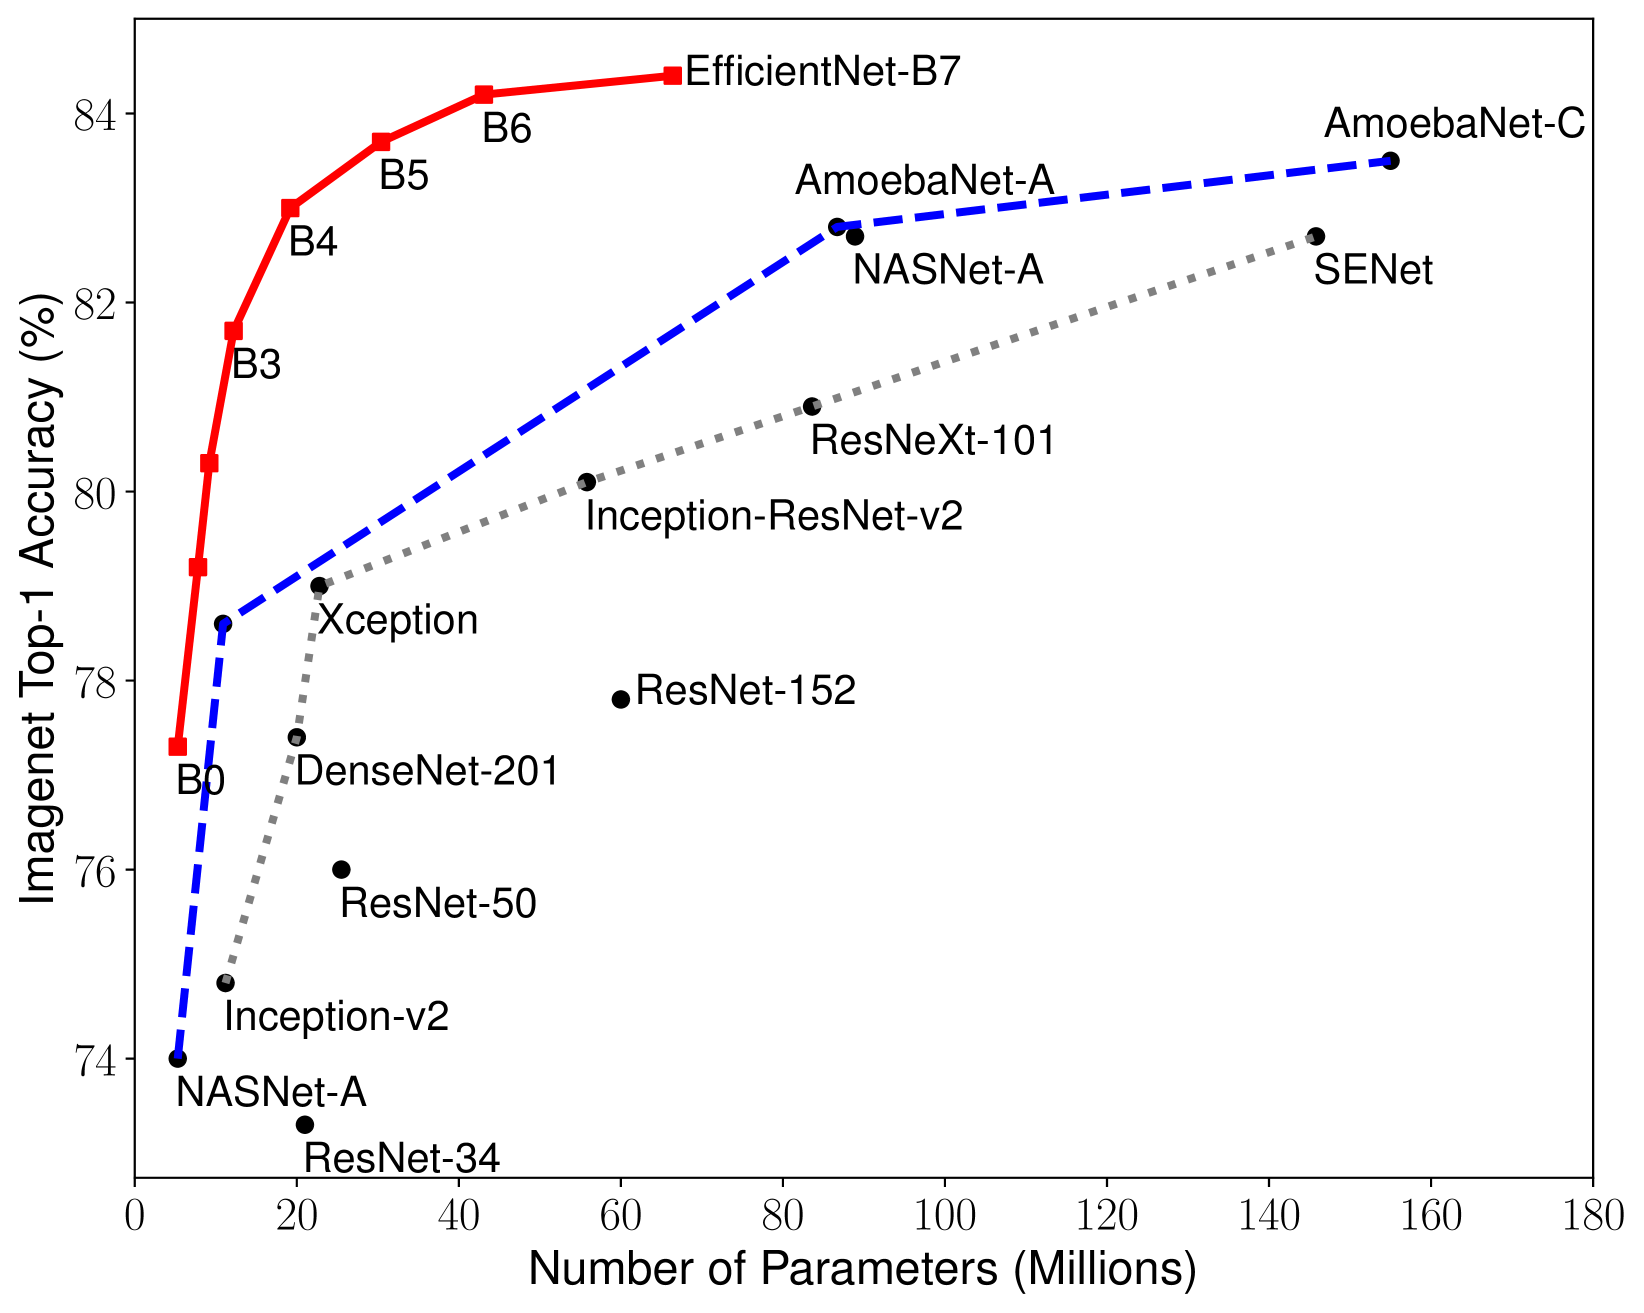
\includegraphics[width=1\textwidth]{./Graphics/efficientnet_performance.png}
      \caption{Estadísticas del rendimiento de los modelos de EfficientNet \brackcite{tan2019efficientnet}.}
      \label{fig:efficientnet_performance}
      \end{center}
      \end{figure}

Los experimentos demostraron que el método de escalado compuesto mejoraba la precisión en modelos ya existentes como MobileNets y ResNet. Los modelos EfficientNet entrenados en ImageNet mostraron una precisión y eficiencia significativamente mayores en comparación con otros ConvNets, utilizando una cantidad mucho menor de parámetros y FLOPS. Especialmente, EfficientNet-B7 logró una precisión del 84.3\% en top-1 en ImageNet, superando modelos anteriores y siendo considerablemente más pequeño y rápido.

En relación con el dataset HAM1000 \brackcite{ham10000}, la implementación del EfficientNetB1 puede ser particularmente beneficiosa para el análisis de datos. EfficientNetB1, entre las variantes de la serie EfficientNet, se encuentra en un punto medio en términos de complejidad y tamaño, ofreciendo un equilibrio entre precisión y eficiencia computacional. Dado que el HAM1000 es un conjunto de datos de imágenes dermatoscópicas que requiere una alta precisión en la identificación y clasificación de lesiones cutáneas, la utilización de EfficientNetB1 podría proporcionar una precisión y eficiencia aceptable en términos de recursos computacionales.

\subsection{Arquitectura del modelo y regularización}

Para fortalecer la arquitectura del modelo, se añadieron capas adicionales, incluyendo \textit{Dropout} y regularizadores L1 y L2, esenciales para combatir el sobre-ajuste. Una capa densa personalizada fue incorporada para facilitar la clasificación precisa de múltiples tipos de tumores. La compilación del modelo se realizó con un enfoque en la clasificación multi-clase, utilizando la pérdida de entropía cruzada categórica (\textit{categorical crossentropy}) y un optimizador \textit{Adamax}.

\subsection{Ajuste dinámico del learning rate}

Un elemento innovador del entrenamiento fue el uso de un \textit{callback} personalizado para el ajuste dinámico del learning rate \brackcite{lr}. Se implementa un mecanismo de ajuste de la tasa de aprendizaje (LRA) personalizado de Keras. Este, ajusta dinámicamente la tasa de aprendizaje durante el entrenamiento basado en la precisión y la pérdida de validación, con el objetivo de mejorar la eficiencia del entrenamiento y alcanzar una mejor convergencia. Los componentes clave del LRA son:

\begin{enumerate}
   \item Modelo: La red neuronal sobre la que se aplicará el \textit{callback}.
   \item Paciencia: El número de épocas que se esperará sin mejora en la métrica de rendimiento antes de realizar un ajuste.
   \item Umbral (\textit{Threshold}): Un valor límite que define cuándo se considera que ha habido una mejora significativa en el rendimiento.
   \item Factor de Ajuste: La magnitud por la cual se modificará el learning rate en caso de no observarse mejoras.
   \item Dwell: Una opción que permite al modelo volver a un estado de pesos anterior si no hay mejoras tras el ajuste del learning rate.
\end{enumerate}

Durante el entrenamiento, el \textit{callback} monitorea constantemente el rendimiento del modelo en términos de precisión y pérdida de validación. Al final de cada época, realiza las siguientes operaciones:

\begin{enumerate}
   \item Evaluación de Métricas: Se revisan la precisión del entrenamiento y la pérdida de validación para determinar si se ha alcanzado o superado el umbral establecido.
   \item Decisión de Ajuste: Basándose en la paciencia y las métricas evaluadas, se decide si se ajustará el learning rate. Si las métricas no han mejorado durante el número de épocas definidas por la paciencia, se procede al ajuste.
   \item Aplicación del Ajuste: Si se requiere un ajuste, el learning rate se multiplica por el factor de ajuste. Este cambio tiene como objetivo reaccionar ante el estancamiento del aprendizaje, estimulando al modelo para explorar nuevas áreas del espacio de parámetros.
   \item Implementación de \textit{Dwell}: En caso de no observarse mejora incluso después del ajuste, y si la opción 'dwell' está activada, el modelo puede revertir a un estado de pesos anterior, evitando así el estancamiento en mínimos locales.
   \item Reporte de Progreso: El callback proporciona información valiosa sobre el progreso del entrenamiento, incluyendo la tasa de aprendizaje actual y la próxima, y si el enfoque está en la precisión o la pérdida de validación.
\end{enumerate}
\chapter{Detalles de implementación y experimentos}\label{chapter:implementation}

\section{Dataset}

El dataset utilizado como medio de aprendizaje para este proyecto es HAM1000-segmentation-and-classification \brackcite{ham10000}. Este conjunto de datos, acrónimo de Human Against Machine (Humano contra máquina) con 10000 imágenes de entrenamiento, es una amplia colección de imágenes dermatoscópicas. En concreto, contiene 10015 imágenes del archivo ISIC, que inicialmente formaban parte de un conjunto de entrenamiento creado por ISIC \brackcite{tschandl2018ham10000} con la siguiente distribución.\\

\begin{tabular}{lrr}
   \hline
   \textbf{Categoría Diagnóstica} & \textbf{Número de Imágenes} & \textbf{Porcentaje} \\
   \hline
   Melanocytic nevi               & 6705                        & 66.95\%             \\
   Melanoma                       & 1113                        & 11.11\%             \\
   Benign keratosis-like lesions  & 1099                        & 10.97\%             \\
   Basal cell carcinoma           & 514                         & 5.13\%              \\
   Actinic keratoses              & 327                         & 3.27\%              \\
   Vascular lesions               & 142                         & 1.42\%              \\
   Dermatofibroma                 & 115                         & 1.15\%              \\
   \hline
   \end{tabular}

\section{Preparación y carga de datos}

Los datos utilizados como medio de aprendizaje para este proyecto son imágenes y metadatos. El dataset HAM10000 contiene imágenes tomadas de varios tipos de cáncer de piel y un archivo de metadatos que contienen información relacionada con cada imagen en formato \textit{one hot encoding}. Esta una técnica de procesamiento de datos en la cual cada valor categórico se representa mediante un vector binario cuyo tamaño corresponde al número de categorías posibles. En dicho vector, todos los elementos son cero, salvo el correspondiente a la categoría del valor, que es uno \brackcite{ohe}

\subsection{Transformación de datos}

Para optimizar la eficiencia del algoritmo, se procesan las imágenes realizando diversas modificaciones, que incluyen: eliminación de cabello, luces y sombras, división de canales y aplicación de un leve desenfoque.

Los metadatos asociados a la clasificación, etiquetados con método mencionado, fueron convertidos a un formato \textit{categórico} \textit{add citation} para su procesamiento. Se define \textit{categórico} como el formato en el que a cada elemento se le asigna el nombre de una categoría como propiedad.

\subsection{Modelación y división del conjunto de datos}

Los datos se modelan a partir de un dataframe de Pandas \brackcite{pandas}. Estos son divididos en 3 conjuntos: Entrenamiento, Validación y Prueba, utilizando un enfoque simple de division de datos en porcentaje. Estas divisiones son necesarias para que el modelo pueda aprender y ser evaluado correctamente.

Inicialmente, el conjunto de datos, fue dividido en dos subconjuntos: \textit{train}, que se destinó para el entrenamiento, y \textit{dummy}, que fue utilizado como una combinación temporal para los conjuntos de validación y prueba. Luego el segundo conjunto fue separado en \textit{valid}, destinado a la validación y \textit{test}, utilizado para las pruebas.

\subsubsection{Experimento 1}

   La distribución de datos fue la siguiente:

   \begin{enumerate}
      \item El 95\% de los datos se destinan al conjunto de entrenamiento.
      \item El 2.5\% de los datos restantes se destinan al conjunto de validación.
      \item El 2.5\% restante se destina al conjunto de pruebas.
   \end{enumerate}
   
   Además se mezclan aleatoriamente los datos y se utiliza una variable fija para garantizar que la división sea reproducible. Aquí se utiliza \textit{dummy split} para mantener la proporción deseada entre validación y prueba.

   \begin{table}[ht]
      \centering
      \begin{tabular}{lccc}
      \hline
      Diagnostic category & Training & Validation & Testing \\ \hline
      AKIEC & 122 & 4 & 1 \\
      BCC & 487 & 12 & 15 \\
      BKL & 1045 & 31 & 23 \\
      DF & 108 & 5 & 2 \\
      MEL & 1036 & 38 & 39 \\
      NV & 6389 & 154 & 162 \\
      VASC & 137 & 1 & 4 \\ \hline
      \end{tabular}
      \caption{Experimento 1: Distribución de imágenes de cáncer de piel en Entrenamiento, Test, y Validación Datasets}
      \label{tab:train_test_validate_e1}
      \end{table}

Por lo que este experimento tiene 9514 datos de entrenamiento, 251 de test y 250 de validación.

\subsubsection{Experimento 2}

La distribución de datos fue la siguiente:

   \begin{enumerate}
      \item El 70\% de los datos se destinan al conjunto de entrenamiento.
      \item El 15\% de los datos restantes se destinan al conjunto de validación.
      \item El 15\% restante se destina al conjunto de pruebas.
   \end{enumerate}
   
Se utiliza \textit{stratify} en ambas divisiones para mantener la distribución de etiquetas \textit{label} en cada conjunto. Se calcula la proporción del conjunto de prueba sobre la suma del conjunto de test y el de validación. 

\begin{table}[ht]
   \centering
   \begin{tabular}{lccc}
   \hline
   Diagnostic category & Training & Validation & Testing \\ \hline
   AKIEC & 88 & 19 & 19 \\
   BCC & 359 & 77 & 77 \\
   BKL & 769 & 164 & 164 \\
   DF & 80 & 17 & 17 \\
   MEL & 779 & 166 & 166 \\
   NV & 4693 & 1005 & 1005 \\
   VASC & 99 & 21 & 21 \\ \hline
   \end{tabular}
   \caption{Experimento 2: Distribución de imágenes de cáncer de piel en los conjuntos de Entrenamiento, Test y Validación}
   \label{tab:train_test_validate_e2}
\end{table}

Luego este quedaría distribuido en 7010 datos de entrenamiento, 1503 de test y 1502 de validación.

\section{Generadores de datos y preprocesamiento}

Uno de los principales problemas del dataset, es el desequilibrio en la representación de las clases, un problema habitual en los conjuntos de datos médicos en los que algunas enfermedades son más raras que otras. Para solucionar este problema, el conjunto de datos se equilibra meticulosamente limitando el número máximo de muestras por clase (300). Esto garantiza que el modelo no esté sesgado hacia las clases más comunes y pueda generalizar mejor entre varios tipos de lesiones cutáneas.

\subsection{Experimento 1}

Se establece para este un tamaño objetivo de muestras por clase (300 en este caso), y se utiliza un bucle para iterar a través de cada clase única. Se realiza un remuestreo con reemplazo para clases con un número de muestras menor al objetivo (300), y sin reemplazo para clases con un número igual o mayor al tamaño objetivo.

\begin{table}[ht]
   \centering
   \begin{tabular}{lccc}
   \hline
   Diagnostic category & Sampling  \\ \hline
   AKIEC & 300 \\
   BCC & 300 \\
   BKL & 300 \\
   DF & 115 \\
   MEL & 300 \\
   NV & 300 \\
   VASC & 142 \\ \hline
   \end{tabular}
   \caption{Distribución de muestras por categoría después del sobre-muestreo}
   \label{tab:sampling_distribution}
   \end{table}


Como se evidencia anteriormente, al separar la data en clases el conjunto se mantiene desbalanceado. Se hace necesario aplicar un método llamado \textit{Class Weighting} \brackcite{analyticsvidhya2020classweight}. Este método se refiere a la asignación de pesos diferenciados a cada clase durante el proceso de entrenamiento del modelo, con el objetivo de reforzar la señal de entrenamiento de las clases menos representadas, o sea, las clases/categorías con menos cantidad de datos:

\begin{table}[ht]
   \centering
   \begin{tabular}{lccc}
   \hline
   Diagnostic category & Sampling  & Weighting\\ \hline
   AKIEC & 300 & 1.00\\
   BCC & 300 & 1.00\\
   BKL & 300 & 1.00\\
   DF & 115 & 2.60\\
   MEL & 300 & 1.00\\
   NV & 300 & 1.00\\
   VASC & 142 & 2.11\\ \hline
   \end{tabular}
   \caption{Distribución de Muestras con peso asignado}
   \label{tab:weighting_distribution}
   \end{table}

\subsection{Experimento 2}

Se establece también un tamaño objetivo de muestras por clase (300). Se utiliza la función \textit{groupby} para agrupar el dataFrame por la etiqueta de clase. Se itera sobre cada grupo, y se realiza un re-muestreo con reemplazo para grupos menores al tamaño deseado y sin reemplazo para los grupos que ya alcanzan o superan el tamaño deseado.

En este, a diferencia del primero, en cada clase se alcanza la misma cantidad de muestras, por lo que no es necesario aplicar \textit{Class Weighting}.

\begin{table}[ht]
   \centering
   \begin{tabular}{lccc}
   \hline
   Diagnostic category & Sampling  \\ \hline
   AKIEC & 300 \\
   BCC & 300 \\
   BKL & 300 \\
   DF & 300 \\
   MEL & 300 \\
   NV & 300 \\
   VASC & 300 \\ \hline
   \end{tabular}
   \caption{Distribución de muestras por categoría después del sobre-muestreo}
   \label{tab:sampling_distribution}
   \end{table}

\subsection{Aumento y división de datos}

Para la carga y procesamiento de imágenes se utilizó la clase ImageDataGenerator de Keras \brackcite{img_gen}. Esta clase es una parte integral de la biblioteca Keras y proporciona una forma eficiente de manipular imágenes para tareas de aprendizaje automático. Su principal función es facilitar la creación de lotes de imágenes que se utilizan durante el entrenamiento y la evaluación de modelos de Machine Learning, especialmente en el contexto de redes neuronales. 

Se inicializa con varias transformaciones (como rotación, desplazamiento y zoom) aplicadas automáticamente a las imágenes a medida que se cargan, para devolver lotes de imágenes listos para el entrenamiento o la evaluación del modelo \brackcite{augmentation}.

\begin{table}[ht]
   \centering
   \begin{tabular}{lccc}
   \hline
   Parámetro & Descripción  & Valor \\ \hline
   rotation range & 	Rango de rotación & 20 grados \\
   width shift range & Rango de desplazamiento horizontal & 20\% \\
   height shift range & Rango de desplazamiento vertical & 20\% \\
   shear range & 	Rango de corte & 20\% \\
   zoom range & Rango de zoom & 20\% \\
   horizontal flip & Activación de volteo horizontal & verdadero \\
   fill mode & Modo de relleno para manejar los píxeles faltantes & nearest \\ \hline
   \end{tabular}
   \caption{Parámetros de aumento de datos}
   \label{tab:data_augmentation_params}
   \end{table}

\section{Diseño y entrenamiento del modelo}

Se utiliza la arquitectura de red neural denominada \textit{EfficientNetB1} \brackcite{efficientnet}. Esta arquitectura forma parte de la familia EfficientNet, que está diseñada para proporcionar alta precisión mientras se mantiene un tamaño de modelo y una complejidad computacional eficientes.

Para aprovechar los conocimientos previos y acelerar el entrenamiento, se carga el modelo \textit{EfficientNetB1} pre-entrenado con los pesos obtenidos al procesar el dataset \textit{ImageNet}. El mismo consiste en una amplia base de datos de imágenes utilizada comúnmente para entrenamiento y \textit{benchmarking} en tareas de visión por computadora. Utilizar este modelo pre-entrenado permite aprovechar las características que ya ha aprendido de este amplio conjunto de datos, facilitando su adaptación al dataset HAM10000.

Se utiliza el \textit{EfficientNetB5} sin incluir su capa superior, con el objetivo de añadir y personalizar capas adicionales. Tras obtener la salida del modelo base, se aplica una serie de transformaciones, incluyendo normalización por lotes, una capa densa con regularizaciones, una técnica de \textit{Dropout} para prevenir el sobre-ajuste y una capa de optimización. 

\subsection{ImageNet}

ImageNet es un proyecto de base de datos visual extenso, diseñado principalmente para la investigación en reconocimiento visual de objetos. Contiene más de 14 millones de imágenes, anotadas manualmente para indicar qué objetos se muestran, y más de 20,000 categorías, cada una con cientos o miles de imágenes. Este proyecto ha sido fundamental en el avance de la visión por computadora y el aprendizaje profundo, proporcionando un recurso de datos inmenso y diverso para entrenar algoritmos de inteligencia artificial.

La relevancia de ImageNet para el aprendizaje profundo se puso de manifiesto con el éxito de AlexNet en el desafío ImageNet 2012 \brackcite{Pinecone2021ImageNet}, donde logró una tasa de error top-5 del 15.3\%, notablemente inferior a la de sus competidores. Este hito marcó un punto de inflexión en el campo, demostrando la viabilidad y la potencia de las redes neuronales convolucionales (CNN) cuando se combinan con unidades de procesamiento gráfico (GPU) para el entrenamiento.

\subsection{Arquitectura del modelo EfficientNet}

La familia de arquitecturas EfficientNet, desarrollada por los autores en \brackcite{tan2019efficientnet}, surgió con el objetivo de hallar un método adecuado para escalar las CNNs de manera que mejoraran tanto en precisión (i.e., rendimiento del modelo) como en eficiencia (es decir, en términos de parámetros del modelo y FLOPS). Estos autores propusieron un método de escalado compuesto que utiliza un conjunto fijo de coeficientes para escalar de manera uniforme el ancho, la profundidad y la resolución de la red. El método les permitió desarrollar una arquitectura de CNN eficiente, a la que denominaron EfficientNet B0. Posteriormente, crearon las variantes EfficientNets B1-B7 escalando la red base (EfficientNet B0).

Mientras que la arquitectura EfficientNet B0 tiene 5.3 millones de parámetros y acepta imágenes de entrada de 224x224, EfficientNet B7 cuenta con 66 millones de parámetros y acepta imágenes de 600x600. \brackcite{Tan2019EfficientNetRM}

\begin{figure}[ht]%
   \begin{center}
   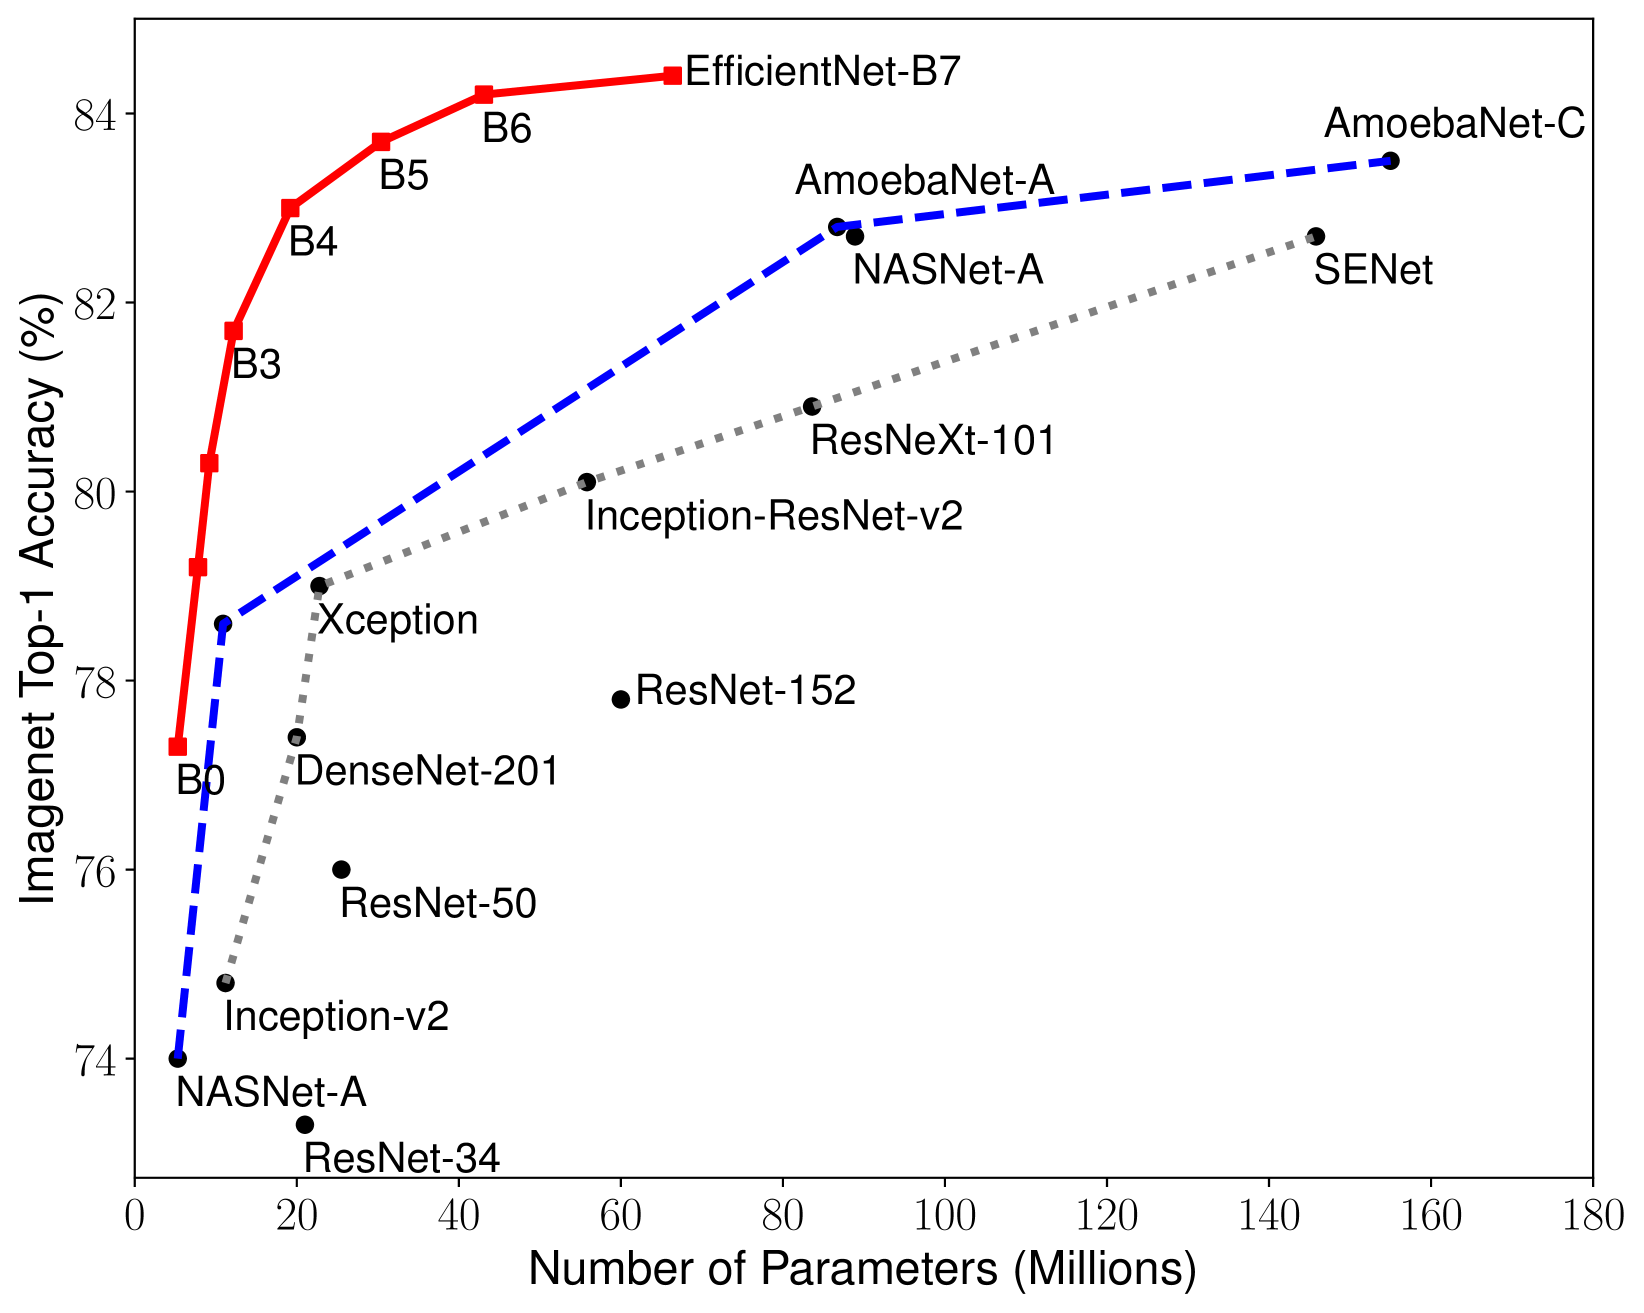
\includegraphics[width=0.45\textwidth]{./Graphics/efficientnet_performance.png}
   \caption{Estadísticas del rendimiento de los modelos de EfficientNet}
   \label{fig:efficientnet_performance}
   \end{center}
   \end{figure}

\subsection{EfficientNetB1}

En relación con el dataset HAM1000 \brackcite{ham10000}, la implementación del EfficientNetB1 puede ser particularmente beneficiosa para el análisis de datos. EfficientNetB1, entre las variantes de la serie EfficientNet, se encuentra en un punto medio en términos de complejidad y tamaño, ofreciendo un equilibrio entre precisión y eficiencia computacional. Dado que el HAM1000 es un conjunto de datos de imágenes dermatoscópicas que requiere una alta precisión en la identificación y clasificación de lesiones cutáneas, la utilización de EfficientNetB5 podría proporcionar una precisión y eficiencia aceptable en términos de recursos computacionales.

\subsection{Capas adicionales y regularización}

Para ajustar el modelo de EfficientNetB1 a nuestras necesidades, se añaden capas adicionales:

\subsubsection{Normalización por lotes}

Para mejorar la estabilidad y eficiencia del modelo EfficientNetB1, se incorpora una capa de Normalización por lotes. La normalización por lotes es crucial para estabilizar las \textit{activaciones} a lo largo de las capas del modelo. Al estandarizar las activaciones por lote, mejora la eficiencia del entrenamiento y permite el uso de tasas de aprendizaje más altas. Esta técnica contribuye significativamente a la regularización del modelo, reduciendo el riesgo de sobre-ajuste y facilitando un aprendizaje más rápido y estable.

Esta capa se define con un \textit{eje de normalización establecido en -1}, lo que indica que la normalización se aplica a lo largo del último eje en el tensor de entrada. Además, se configura un \textit{momentum} de $0.99$ y un valor de \textit{epsilon} de $0.001$. El alto valor de momentum ayuda a mantener la estabilidad de las medias y varianzas móviles a lo largo del entrenamiento, mientras que el pequeño valor de epsilon evita divisiones por cero, asegurando así cálculos numéricos estables. [\brackcite{regularization}]

\subsubsection{Capa densa}

Se integra una capa densa con $256$ neuronas, que juega un papel clave en la síntesis de las características aprendidas por el modelo. Se utiliza un regularizador \textit{L2} con un \textit{lambda} de $0.016$ para los pesos de la capa, lo que ayuda a penalizar y controlar el tamaño de los pesos, reduciendo así el riesgo de sobre-ajuste. Además, tanto el regularizador de actividad como el regularizador de bias se configuran con un regularizador \textit{L1} con un \textit{lambda} de $0.006$. Este enfoque impone una penalización en los pesos y los sesgos, promoviendo un modelo más simple y disperso. La función de activación utilizada es \textit{ReLU} , conocida por su eficacia en la introducción de no linealidad en el modelo, lo que permite aprender relaciones complejas entre las características. \brackcite{dense}

\subsubsection{Dropout}

En la arquitectura del modelo, se integra una capa de dropout para aumentar la robustez y prevenir el sobre-ajuste. Esta capa se configura con una tasa de desactivación del 45\% , lo que significa que, durante el entrenamiento, el 45\% de las neuronas se desactivarán aleatoriamente en cada paso. 

En una primera iteración del algoritmo tuvo una tasa de desactivación más baja. Luego de varias iteraciones se concluyó que se necesitaba un algoritmo de clasificación que estudiara más a detalle la data fomentando así una mejor generalización y reduciendo el riesgo de sobre-ajuste en el proceso de aprendizaje. Basándonos en esto aumentamos la tasa y obtuvimos mejores resultados.

Para asegurar la reproducibilidad, se establece una semilla(seed) $123$. Esta introducción de aleatoriedad ayuda a que el modelo no dependa excesivamente de ninguna característica o neurona específica. \brackcite{dropout}

\subsubsection{Capa de salida}

La capa de salida utiliza una activación \textit{softmax} para transformar las salidas del modelo en probabilidades de pertenencia a cada clase. Esto, clasifica las entradas en categorías distintas, proporcionando probabilidades para cada clase, lo cual es esencial en la clasificación multi-clase.

\subsection{Optimización}

Para el proceso de entrenamiento, se utiliza el optimizador \textit{Adamax} \brackcite{adamax}. Este es una variante del conocido optimizador Adam, que combina las ventajas de los métodos adaptativos de tasa de aprendizaje con una implementación más robusta en entornos con gradientes dispersos, lo cual es común en imágenes médicas 

La función de pérdida elegida es la \textit{categorical crossentropy} \brackcite{vitalflux_categorical_crossentropy}, idónea para problemas de clasificación multi-clase. Se configura el modelo para minimizarla y se rastrea la precisión como métrica principal.

\subsection{Ajuste dinámico de la tasa de aprendizaje}

Un componente innovador de nuestro enfoque es el uso de un Callback personalizado para el ajuste dinámico del learning rate \brackcite{lr}, basado en la precisión del entrenamiento y la pérdida de validación. Este mecanismo adapta el learning rate durante el entrenamiento, reduciéndolo si el modelo no mejora a un ritmo esperado. Este ajuste es vital en la navegación de superficies de pérdida complejas, aumentando la probabilidad de que el modelo evite mínimos locales subóptimos y converja hacia soluciones más efectivas.

%-----------------------------------------------------------------------------------
\section{Resultados}\label{sec:results}
%-----------------------------------------------------------------------------------

En esta sección presentamos los resultados obtenidos. Nuestro enfoque se centró en la exploración y optimización de dos pipelines de procesamiento y clasificación de imágenes. Los experimentos se estructuraron con el objetivo de evaluar mejoras de precisión en el modelo utilizando distintas aproximaciones de procesamiento y normalización de datos y optimizadores en el contexto del procesamiento de imágenes.

Tras la implementación del modelo, los resultados obtenidos superan las espectativas. El modelo con mayor eficiencia luego de varios ajustes tuvo una eficacia de validación cercana al 84\%. Los resultados son un paso significativo hacia la automatización del diagnóstico del cáncer de piel, que tradicionalmente ha dependido de la inspección visual por parte de expertos humanos. 

En cada sección se muestran algunas métricas que muestran el desarrollo del modelo, con los siguientes parámetros:

\begin{table}[ht]
   \centering
   \small
   \begin{tabular}{|c|p{10cm}|}
   \hline
   \textbf{Término} & \textbf{Descripción} \\
   \hline
   Epoch & Es una iteración completa sobre todo el conjunto de datos de entrenamiento. \\
   \hline
   Loss (Pérdida) & Es una medida de cuán bien el modelo está realizando sus predicciones. Los valores decrecientes indican una mejora en el aprendizaje. \\
   \hline
   Accuracy (Precisión) & Muestra el porcentaje de etiquetas que el modelo predice correctamente para el conjunto de entrenamiento. \\
   \hline
   V loss (Pérdida de Validación) & Es similar a la pérdida, pero se calcula sobre un conjunto de datos que no se utiliza para el entrenamiento. \\
   \hline
   V acc (Precisión de Validación) & Muestra el porcentaje de etiquetas que el modelo predice correctamente para el conjunto de datos de validación. \\
   \hline
   LR (Learning Rate) & La tasa de aprendizaje dicta cuánto se ajustan los pesos del modelo en cada actualización. \\
   \hline
   Next LR (Próxima Learning Rate) & Indica la próxima tasa de aprendizaje planificada. La adaptación de la tasa de aprendizaje puede ayudar a evitar el estancamiento y mejorar la convergencia. \\
   \hline
   Monitor & Muestra la métrica que se está utilizando para monitorizar el rendimiento del modelo. Cambia de \textit{accuracy} a \textit{val loss}, lo que probablemente indica que el cambio se hizo para evitar el sobre'ajuste. \\
   \hline
   Duration (Duración) & Tiempo que tardó cada epoch en completarse. Importante para evaluar la eficiencia del entrenamiento. \\
   \hline
   \end{tabular}
   \caption{Descripción de términos clave en el entrenamiento de modelos de aprendizaje automático.}
   \label{table:terminology}
   \end{table}
   

\subsection{Experimento 1}

%-----------------------------------------------------------------------------------
	\subsubsection{Estadísticas básicas}\label{sub:basic_statistics_p1}
%-----------------------------------------------------------------------------------
    
    Estos resultados de la tabla siguiente corresponden a la evaluación del modelo a lo largo de 40 epochs (o iteraciones) de entrenamiento.

    \begin{figure}[ht]
      \small
      \begin{center}
          \begin{tabular}{|c|c|c|c|c|c|c|c|} \hline
          E & Loss & Acc & V loss & V acc & LR & M & Batch \\ \hline
          1 & 9.587 & 40.581 & 8.95658 & 56.800 & $10^{-2}$ & accuracy & 85.25 \\ \hline
          2 & 7.798 & 67.615 & 7.67235 & 66.800 & $10^{-2}$ & accuracy & 21.72 \\ \hline
          3 & 6.884 & 79.340 & 6.96014 & 69.600 & $10^{-2}$ & accuracy & 22.56 \\ \hline
          4 & 6.214 & 87.365 & 6.35865 & 71.200 & $10^{-2}$ & accuracy & 25.81 \\ \hline
          5 & 5.646 & 91.690 & 5.94812 & 75.200 & $10^{-2}$ & val\_loss & 23.08 \\ \hline
          6 & 5.172 & 92.999 & 5.44954 & 76.800 & $10^{-2}$ & val\_loss & 23.23 \\ \hline
          7 & 4.735 & 94.479 & 5.06016 & 76.400 & $10^{-2}$ & val\_loss & 23.19 \\ \hline
          8 & 4.334 & 96.528 & 4.73837 & 76.800 & $10^{-2}$ & val\_loss & 22.90 \\ \hline
          9 & 3.969 & 97.211 & 4.33689 & 77.200 & $10^{-2}$ & val\_loss & 22.74 \\ \hline
          10 & 3.631 & 98.008 & 4.15826 & 74.000 & $10^{-2}$ & val\_loss & 22.56 \\ \hline
          11 & 3.315 & 98.406 & 3.89153 & 73.600 & $10^{-2}$ & val\_loss & 23.11 \\ \hline
          \dots & \dots & \dots & \dots & \dots & \dots & \dots & \dots \\ \hline
          34 & 0.627 & 99.886 & 1.24470 & 76.800 & 0.00013 & val\_loss & 23.30 \\ \hline
          \end{tabular}
          \caption{Estadísticas básicas del modelo EfficientNetB1.}
      \end{center}\label{fig:estadisticas_p1}
  \end{figure}
    
  Aquí vemos que el entrenamiento se planeó para 40 epochs, pero se detuvo en el epoch 34, después de tres ajustes de la tasa de aprendizaje sin mejoras en la pérdida de validación. Esto ocurre dado que el modelo no estaba mejorando su capacidad de generalizar a datos no vistos y que continuar el entrenamiento probablemente habría resultado en un gasto innecesario de recursos y posiblemente en un mayor sobre-ajuste. 
  
  En la tabla se observa que la precisión de entrenamiento aumenta con cada epoch, la pérdida de entrenamiento disminuye consistentemente, la tasa de aprendizaje permanece constante al principio y luego disminuye para afinar el entrenamiento a medida que el modelo comienza a converger, todo lo anterior es indicador que el modelo esta entrenando de forma correcta.

  En el monitor se muestra que cambia de \textit{accuracy} a \textit{val loss}, este cambio se hizo para evitar el sobre-ajuste.

%-----------------------------------------------------------------------------------
\subsubsection{Estadísticas de aprendizaje}\label{sub:learning_statistics_p1}
%-----------------------------------------------------------------------------------
		\begin{figure}[ht]%
      \begin{center}
      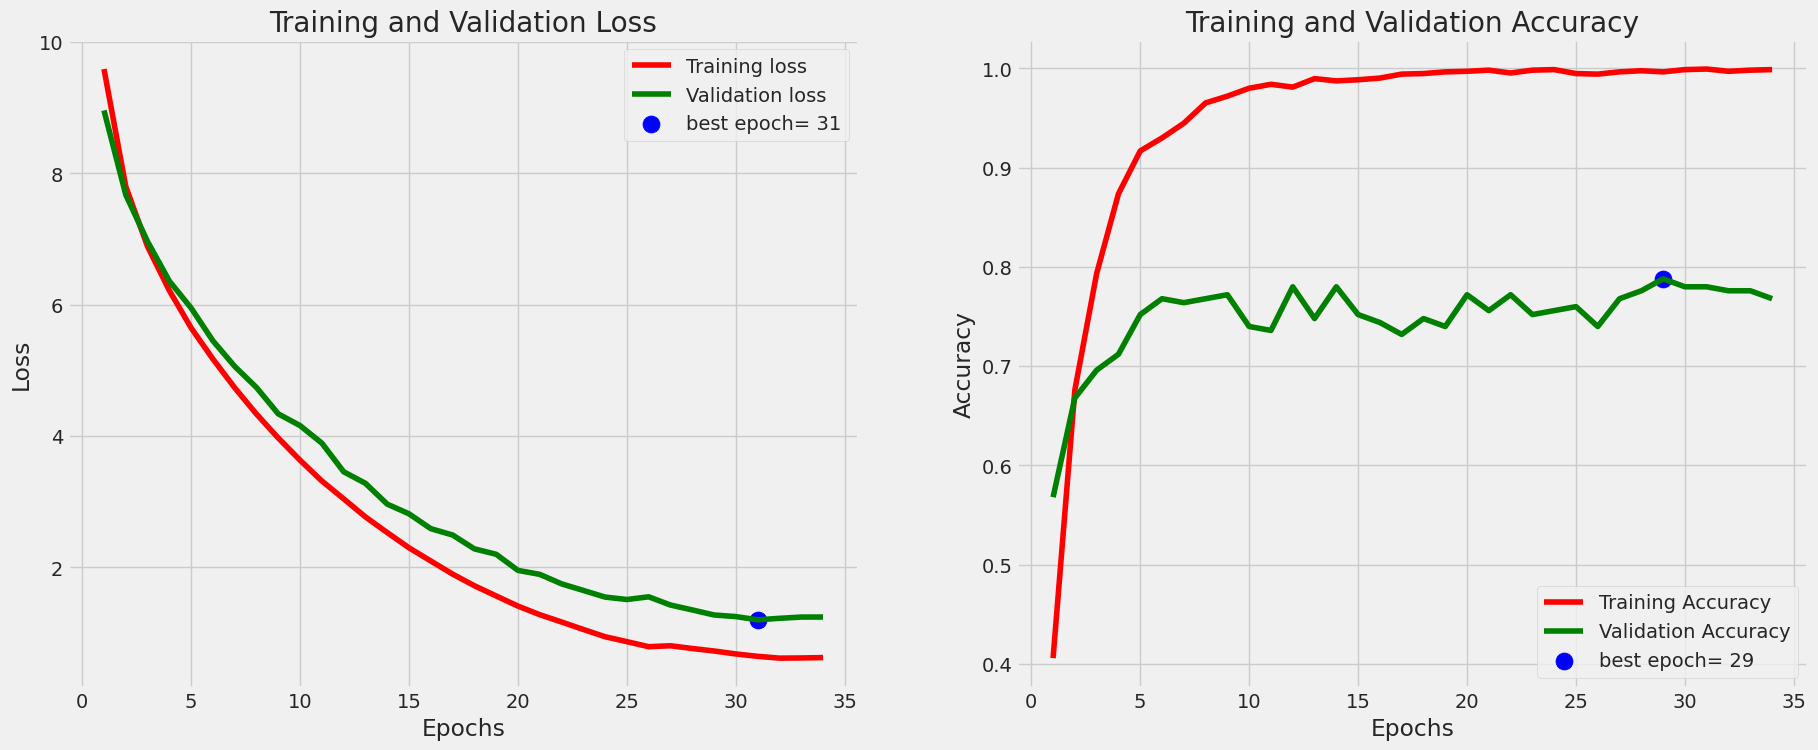
\includegraphics[width=1\textwidth]{./Graphics/training&validation_p1.png}
      \caption{Estadísticas de aprendizaje a lo largo del proceso de entrenamiento.\label{fig:training_validation_loss}}
      \end{center}
		\end{figure}
  
La imagen anterior muestra dos gráficos, uno de pérdida y otro de precisión respectivamente, a lo largo de los epochs de entrenamiento y validación. El primero muestra una disminución constante de la pérdida tanto en el entrenamiento como en la validación, lo cual es indicativo de un buen aprendizaje. La pérdida de validación tiene un mínimo en el epoch 31, lo que sugiere que este podría ser el mejor modelo para evitar el sobre-ajuste. A partir de este punto, si la pérdida de validación comenzase a aumentar mientras la pérdida de entrenamiento sigue disminuyendo, indicaría sobre-ajuste.

En el segundo se aprecia como la precisión de entrenamiento aumenta rápidamente y luego se estabiliza cerca del 100\%, mientras que la precisión de validación también aumenta pero con cierta variabilidad entre los epochs. El mejor epoch según la precisión de validación es el 29. Esta diferencia entre la precisión de entrenamiento y de validación sugiere que puede haber variabilidad en los datos de validación.

%-----------------------------------------------------------------------------------
	\subsubsection{Estadísticas de eficacia}\label{sub:accuracy_statistic_p1}
%-----------------------------------------------------------------------------------
    La matriz de confusión proporciona información valiosa sobre el rendimiento del modelo en relación de Actual/Predicho, en términos de su capacidad para clasificar correctamente cada una de las siete clases de cáncer de piel. La diagonal principal de la matriz representa los verdaderos positivos (TP), el número de casos en los que el modelo ha predicho correctamente la clase correspondiente. Los valores fuera de la diagonal principal indican errores de clasificación.

    La clase 'NV' muestra una alta cantidad de clasificaciones correctas (134), pero también tiene errores significativos al ser confundida con otras clases (como 'BKL' y 'MEL'). La clase 'AKIEC' resultó la más difícil de predecir, con la mayoría de las muestras mal clasificadas. Esto puede deberse a la similitud entre las características de estas clases, pero sobre todo al desbalance en el conjunto de datos.
    
    \begin{figure}[ht]%
		\begin{center}
		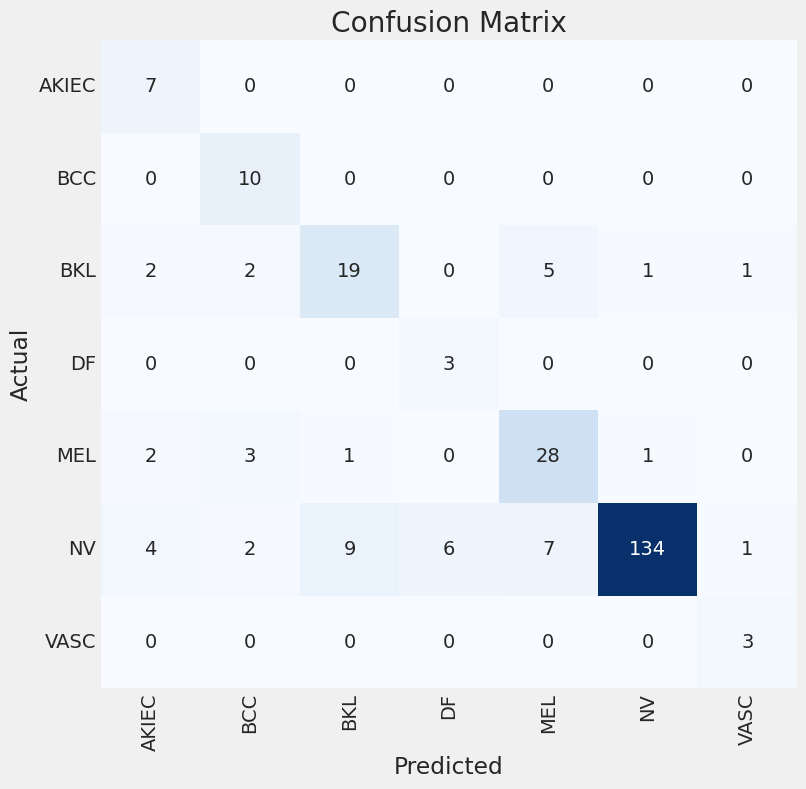
\includegraphics[width=1\textwidth]{./Graphics/confussionmatrix_p1.png}
		\caption{Estadísticas de eficacia del modelo al estimar los resultados en el conjunto de pruebas\label{fig:confussion_matrix_p1}}
		\end{center}
		\end{figure}

      \begin{figure}[ht]%
         \begin{center}
         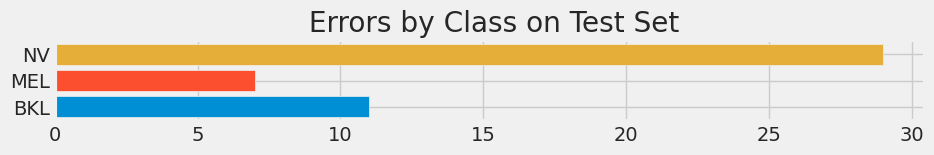
\includegraphics[width=1\textwidth]{./Graphics/errorByClass_p1.png}
         \caption{Gráfico de errores por clase en el conjunto de pruebas\label{fig:class_errors_p1}}
         \end{center}
         \end{figure}

         Cada barra representa el número de muestras de una clase particular que fueron mal clasificadas.
\subsection{Experimento 2}

%-----------------------------------------------------------------------------------
\subsection{Estadísticas básicas}\label{sub:basic_statistics_p2}
%-----------------------------------------------------------------------------------
    
    Estos resultados de la tabla siguiente corresponden a la evaluación del modelo a lo largo de 40 epochs (o iteraciones) de entrenamiento. Cada fila representa una época y se presentan las siguientes métricas:
    
    \begin{figure}[ht]
      \small
      \begin{center}
          \begin{tabular}{|c|c|c|c|c|c|c|c|} \hline
          E & Loss & Acc & V loss & V acc & LR & M & Batch \\ \hline
          1 & 9.587 & 40.581 & 8.95658 & 56.800 & $10^{-2}$ & accuracy & 85.25 \\ \hline
          2 & 7.798 & 67.615 & 7.67235 & 66.800 & $10^{-2}$ & accuracy & 21.72 \\ \hline
          3 & 6.884 & 79.340 & 6.96014 & 69.600 & $10^{-2}$ & accuracy & 22.56 \\ \hline
          4 & 6.214 & 87.365 & 6.35865 & 71.200 & $10^{-2}$ & accuracy & 25.81 \\ \hline
          5 & 5.646 & 91.690 & 5.94812 & 75.200 & $10^{-2}$ & val\_loss & 23.08 \\ \hline
          6 & 5.172 & 92.999 & 5.44954 & 76.800 & $10^{-2}$ & val\_loss & 23.23 \\ \hline
          7 & 4.735 & 94.479 & 5.06016 & 76.400 & $10^{-2}$ & val\_loss & 23.19 \\ \hline
          8 & 4.334 & 96.528 & 4.73837 & 76.800 & $10^{-2}$ & val\_loss & 22.90 \\ \hline
          9 & 3.969 & 97.211 & 4.33689 & 77.200 & $10^{-2}$ & val\_loss & 22.74 \\ \hline
          10 & 3.631 & 98.008 & 4.15826 & 74.000 & $10^{-2}$ & val\_loss & 22.56 \\ \hline
          11 & 3.315 & 98.406 & 3.89153 & 73.600 & $10^{-2}$ & val\_loss & 23.11 \\ \hline
          \dots & \dots & \dots & \dots & \dots & \dots & \dots & \dots \\ \hline
          34 & 0.627 & 99.886 & 1.24470 & 76.800 & 0.00013 & val\_loss & 23.30 \\ \hline
          \end{tabular}
          \caption{Estadísticas básicas de algunas iteraciones del modelo EfficientNetB5.}
      \end{center}\label{fig:estadisticas_p2}
  \end{figure}
    
    En general, los resultados muestran que el modelo mejora con el tiempo, ya que la pérdida disminuye y la precisión aumenta tanto en el conjunto de datos de entrenamiento como en el de validación.

%-----------------------------------------------------------------------------------
\subsection{Estadísticas de aprendizaje}\label{sub:learning_statistics_p2}
%-----------------------------------------------------------------------------------
		\begin{figure}[ht]%
      \begin{center}
      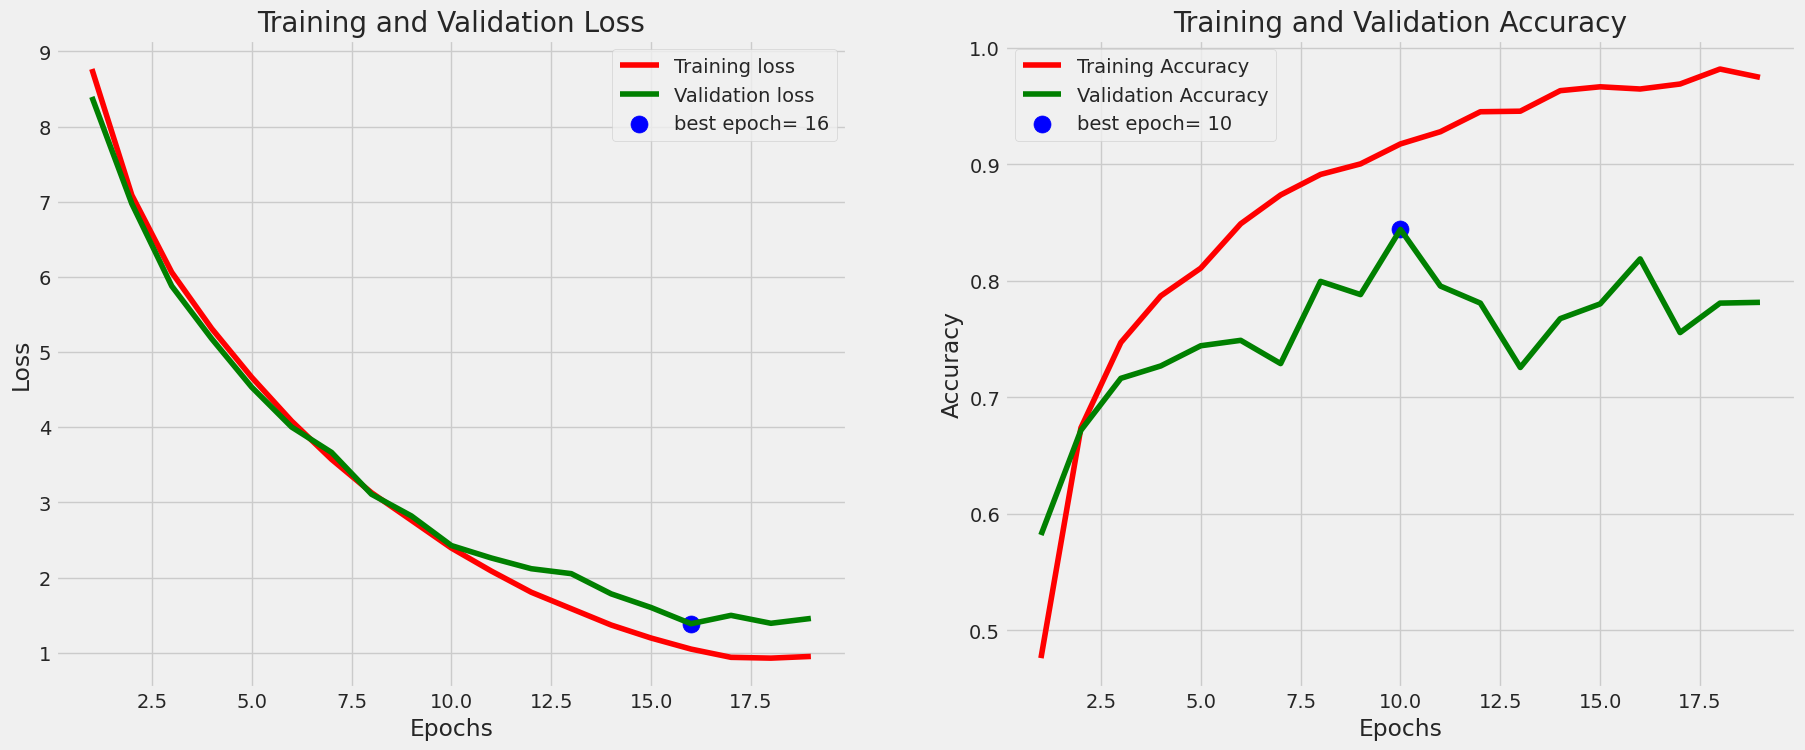
\includegraphics[width=1\textwidth]{./Graphics/training&validation_p2.png}
      \caption{Estadísticas de aprendizaje a lo largo del proceso de entrenamiento.\label{fig:training_validation_loss_p2}}
      \end{center}
		\end{figure}
  
La época con la mejor pérdida de validación y la mejor precisión de validación no coinciden, sugiere un trade-off entre la optimización de la pérdida y la maximización de la precisión. La volatilidad en la precisión de validación sugiere que el modelo puede beneficiarse de un ajuste en el tamaño del lote para suavizar las actualizaciones de los pesos y mejorar la estabilidad del modelo.

Dado lo anterior, se hizo una última iteración del modelo aumentando el volumen de muestras por clase a 500. Estos fueron los resultados. Se obtuvo una efectividad de aproximadamente 87\% (86.83\%).

\begin{figure}[ht]%
   \begin{center}
   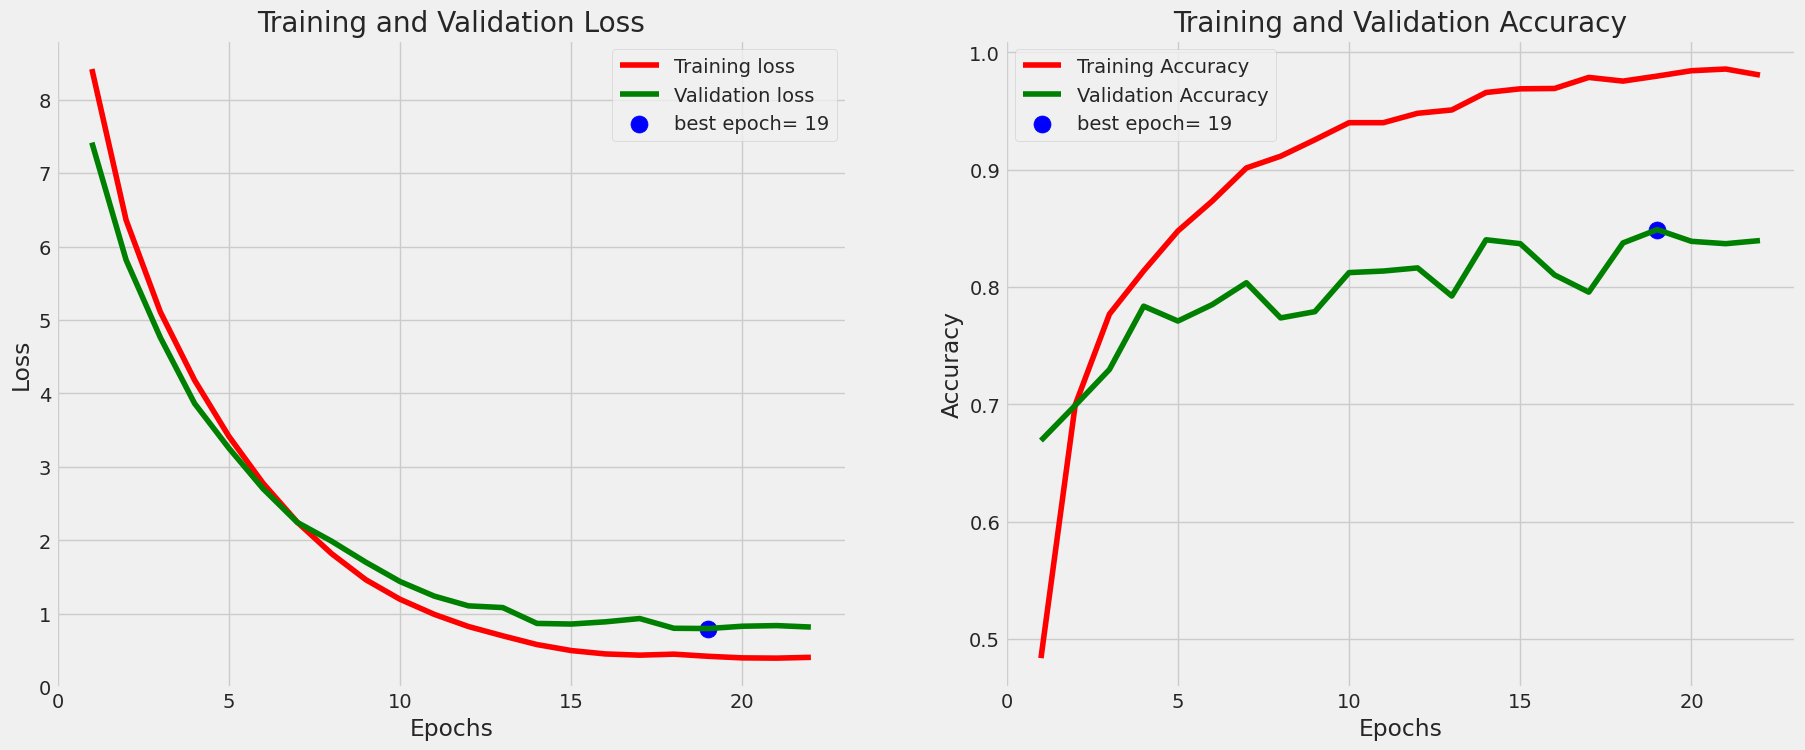
\includegraphics[width=1\textwidth]{./Graphics/training&validation_p3.png}
   \caption{Estadísticas de aprendizaje a lo largo del proceso de entrenamiento.\label{fig:training_validation_loss_p3}}
   \end{center}
   \end{figure}

La disminución continua en la pérdida de entrenamiento y la tendencia ascendente en la precisión de entrenamiento sugieren que el modelo está aprendiendo de manera efectiva y consistente. La pérdida de validación que converge con la de entrenamiento y la mejor época coincidente para pérdida y precisión de validación (época 19) indican que el modelo generaliza bien y no solo memoriza los datos de entrenamiento.

En el gráfico actual, hay una mejor alineación entre la pérdida de entrenamiento y validación y menos volatilidad en la precisión de validación, lo que indica un modelo más estable.

%-----------------------------------------------------------------------------------
	\subsection{Estadísticas de eficacia}\label{sub:accuracy_statistic_p2}
%-----------------------------------------------------------------------------------
    
\begin{figure}[ht]%
   \begin{center}
   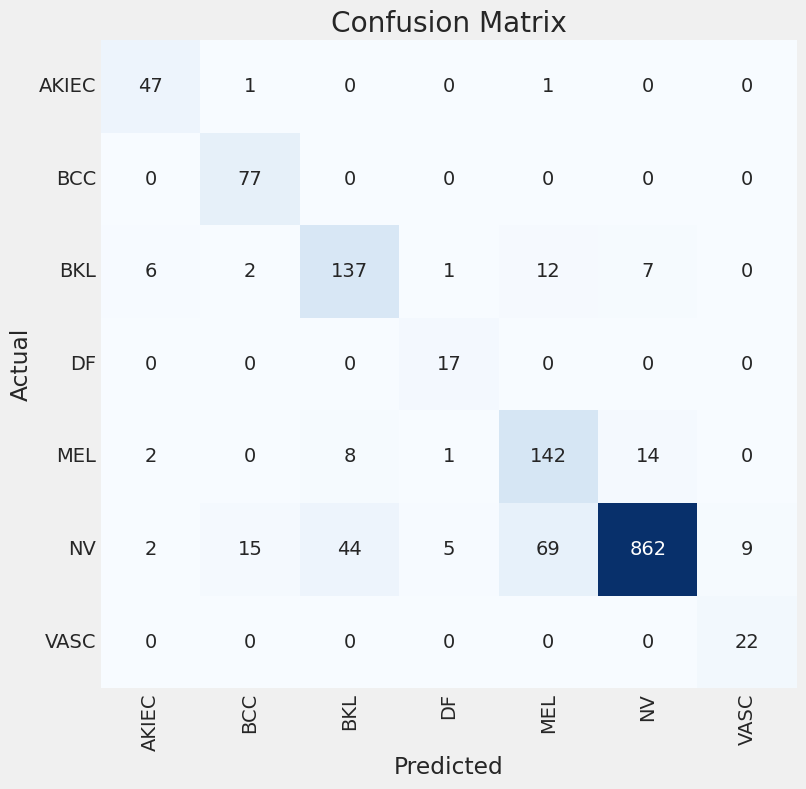
\includegraphics[width=1\textwidth]{./Graphics/confussionMatrix_p3.png}
   \caption{Estadísticas de eficacia del modelo al estimar los resultados en el conjunto de pruebas\label{fig:confussion_matrix_p3}}
   \end{center}
   \end{figure}

   \begin{figure}[ht]%
      \begin{center}
      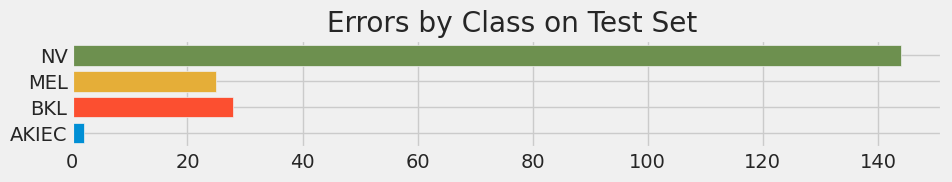
\includegraphics[width=1\textwidth]{./Graphics/errorByClass_p3.png}
      \caption{Gráfico de errores por clase en el conjunto de pruebas\label{fig:class_errors_p3}}
      \end{center}
      \end{figure}

NV muestra la mayoría de los errores, lo que puede deberse a una mayor prevalencia en el conjunto de datos.

Comparando ambos gráficos, podemos identificar áreas específicas donde el modelo necesita mejora. Por ejemplo, la clase 'NV', a pesar de tener muchas predicciones correctas, tiene un número relativamente alto de falsos positivos y falsos negativos, lo que sugiere que puede haber características de las imágenes 'NV' que se confunden con otras clases. En cambio, 'BCC' y 'DF' parecen estar bien diferenciados del resto. Esto puede informar estrategias futuras para mejorar la precisión del modelo, como la recolección de más datos o la implementación de técnicas de aprendizaje más avanzadas para clases específicas.
\chapter{Resultados}\label{chapter:results}

En esta sección presentamos los resultados obtenidos. Nuestro enfoque se centró en la exploración y optimización de dos pipelines de procesamiento y clasificación de imágenes. Los experimentos se estructuraron con el objetivo de evaluar mejoras de precisión en el modelo utilizando distintas aproximaciones de división y normalización de datos en el contexto del procesamiento de imágenes.

El modelo con mayor eficiencia luego de varios ajustes tuvo una eficacia de validación cercana al 84\%. Los resultados son un paso significativo hacia la automatización del diagnóstico del cáncer de piel, que tradicionalmente ha dependido de la inspección visual por parte de expertos humanos. 

En cada sección se muestran algunas métricas que muestran el desarrollo del modelo, con los siguientes parámetros:

\begin{table}[ht]
   \centering
   \small
   \begin{tabular}{|c|p{10cm}|}
   \hline
   \textbf{Término} & \textbf{Descripción} \\
   \hline
   Epoch & Es una iteración completa sobre todo el conjunto de datos de entrenamiento. \\
   \hline
   Loss (Pérdida) & Es una medida de cuán bien el modelo está realizando sus predicciones. Los valores decrecientes indican una mejora en el aprendizaje. \\
   \hline
   Accuracy (Precisión) & Muestra el porcentaje de etiquetas que el modelo predice correctamente para el conjunto de entrenamiento. \\
   \hline
   V loss (Pérdida de Validación) & Es similar a la pérdida, pero se calcula sobre un conjunto de datos que no se utiliza para el entrenamiento. \\
   \hline
   V acc (Precisión de Validación) & Muestra el porcentaje de etiquetas que el modelo predice correctamente para el conjunto de datos de validación. \\
   \hline
   LR (Learning Rate) & La tasa de aprendizaje dicta cuánto se ajustan los pesos del modelo en cada actualización. \\
   \hline
   Next LR (Próxima Learning Rate) & Indica la próxima tasa de aprendizaje planificada. La adaptación de la tasa de aprendizaje puede ayudar a evitar el estancamiento y mejorar la convergencia. \\
   \hline
   Monitor & Muestra la métrica que se está utilizando para monitorizar el rendimiento del modelo. Cambia de \textit{accuracy} a \textit{val loss}, lo que probablemente indica que el cambio se hizo para evitar el sobre'ajuste. \\
   \hline
   Duration (Duración) & Tiempo que tardó cada epoch en completarse. Importante para evaluar la eficiencia del entrenamiento. \\
   \hline
   \end{tabular}
   \caption{Descripción de términos clave en el entrenamiento de modelos de aprendizaje automático.}
   \label{table:terminology}
   \end{table}
   

\section{Experimento 1: Evaluación de la eficiencia de la división asimétrica de datos en la clasificación de imágenes de cáncer de piel}\label{subsec:exp1}


%-----------------------------------------------------------------------------------
\subsection*{Estadísticas básicas}\label{sub:basic_statistics_p1}
%-----------------------------------------------------------------------------------
    
    Estos resultados de la tabla siguiente corresponden a la evaluación del modelo a lo largo de 40 epochs (iteraciones) de entrenamiento.

    \begin{figure}[ht]
      \small
      \begin{center}
          \begin{tabular}{|c|c|c|c|c|c|c|c|} \hline
          E & Loss & Acc & V loss & V acc & LR & M & Batch \\ \hline
          1 & 9.587 & 40.581 & 8.95658 & 56.800 & $10^{-2}$ & accuracy & 85.25 \\ \hline
          2 & 7.798 & 67.615 & 7.67235 & 66.800 & $10^{-2}$ & accuracy & 21.72 \\ \hline
          3 & 6.884 & 79.340 & 6.96014 & 69.600 & $10^{-2}$ & accuracy & 22.56 \\ \hline
          4 & 6.214 & 87.365 & 6.35865 & 71.200 & $10^{-2}$ & accuracy & 25.81 \\ \hline
          5 & 5.646 & 91.690 & 5.94812 & 75.200 & $10^{-2}$ & val\_loss & 23.08 \\ \hline
          6 & 5.172 & 92.999 & 5.44954 & 76.800 & $10^{-2}$ & val\_loss & 23.23 \\ \hline
          7 & 4.735 & 94.479 & 5.06016 & 76.400 & $10^{-2}$ & val\_loss & 23.19 \\ \hline
          8 & 4.334 & 96.528 & 4.73837 & 76.800 & $10^{-2}$ & val\_loss & 22.90 \\ \hline
          9 & 3.969 & 97.211 & 4.33689 & 77.200 & $10^{-2}$ & val\_loss & 22.74 \\ \hline
          10 & 3.631 & 98.008 & 4.15826 & 74.000 & $10^{-2}$ & val\_loss & 22.56 \\ \hline
          11 & 3.315 & 98.406 & 3.89153 & 73.600 & $10^{-2}$ & val\_loss & 23.11 \\ \hline
          \dots & \dots & \dots & \dots & \dots & \dots & \dots & \dots \\ \hline
          34 & 0.627 & 99.886 & 1.24470 & 76.800 & 0.00013 & val\_loss & 23.30 \\ \hline
          \end{tabular}
          \caption{Estadísticas básicas del modelo EfficientNetB1.}
      \end{center}\label{fig:estadisticas_p1}
  \end{figure}
    
  Aquí vemos que el entrenamiento se planeó para 40 epochs, pero se detuvo en el epoch 34, después de tres ajustes de la tasa de aprendizaje sin mejoras en la pérdida de validación. Esto ocurre dado que el modelo no estaba mejorando su capacidad de generalizar a datos no vistos y que continuar el entrenamiento probablemente habría resultado en un gasto innecesario de recursos y posiblemente en un mayor sobre-ajuste. 
  
  En la tabla se observa que la precisión de entrenamiento aumenta con cada epoch, la pérdida de entrenamiento disminuye consistentemente, la tasa de aprendizaje permanece constante al principio y luego disminuye para afinar el entrenamiento a medida que el modelo comienza a converger, todo lo anterior es indicador que el modelo esta entrenando de forma correcta.

  En el monitor se muestra que cambia de \textit{accuracy} a \textit{val loss}, este cambio se hizo para evitar el sobre-ajuste.

%-----------------------------------------------------------------------------------
\subsection*{Estadísticas de aprendizaje}\label{sub:learning_statistics_p1}
%-----------------------------------------------------------------------------------
		\begin{figure}[ht]%
      \begin{center}
      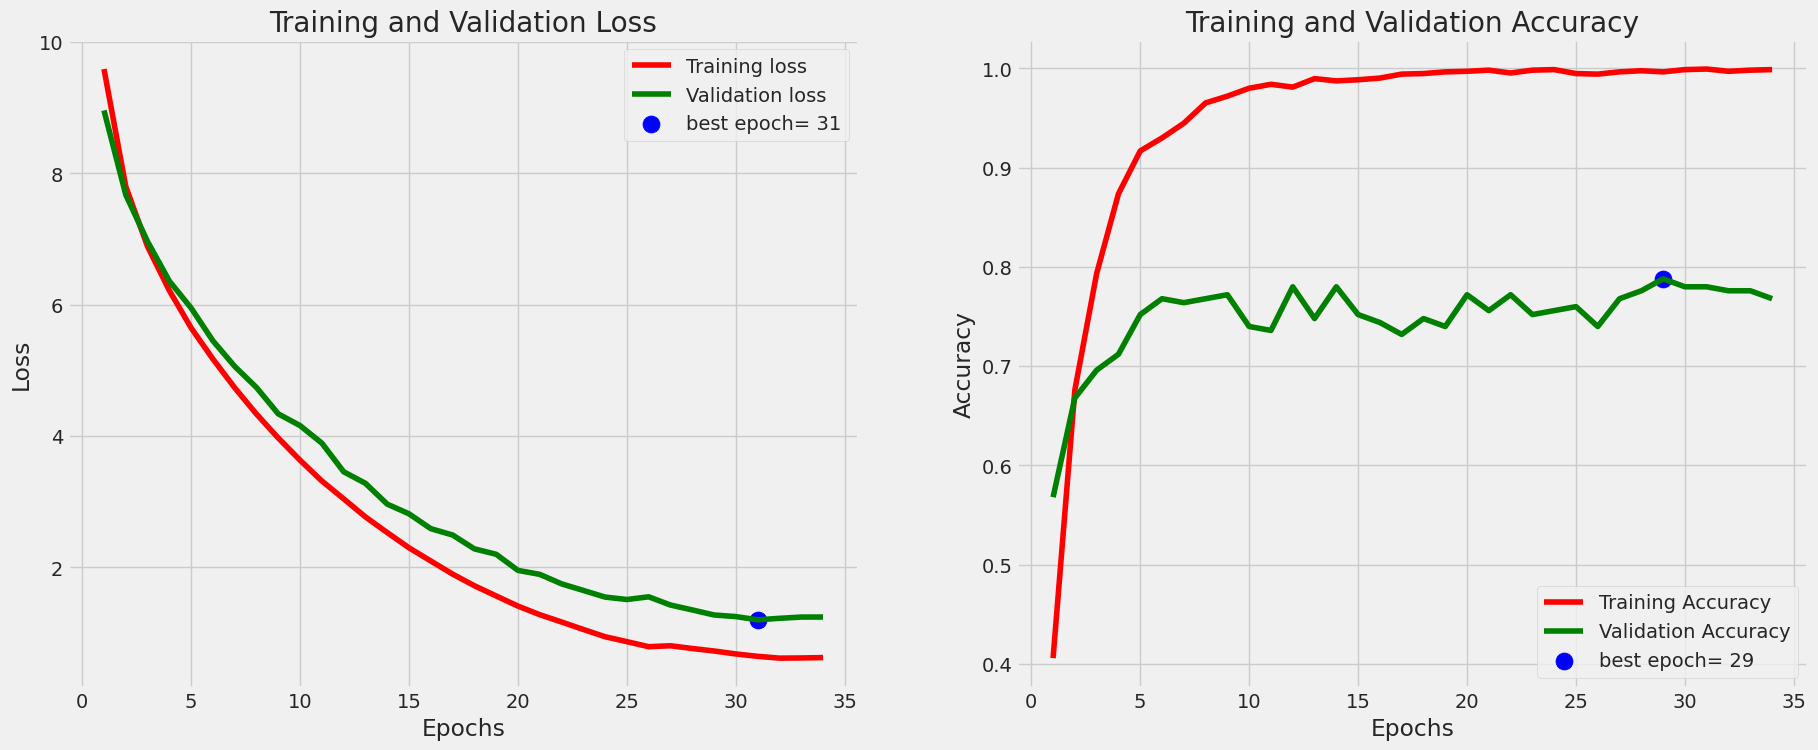
\includegraphics[width=1\textwidth]{./Graphics/training&validation_p1.png}
      \caption{Estadísticas de aprendizaje a lo largo del proceso de entrenamiento.\label{fig:training_validation_loss}}
      \end{center}
		\end{figure}
  
La imagen anterior muestra dos gráficos, uno de pérdida y otro de precisión respectivamente, a lo largo de los epochs de entrenamiento y validación. El primero muestra una disminución constante de la pérdida tanto en el entrenamiento como en la validación, lo cual es indicativo de un buen aprendizaje. La pérdida de validación tiene un mínimo en el epoch 31, lo que sugiere que este podría ser el mejor modelo para evitar el sobre-ajuste. A partir de este punto, si la pérdida de validación comenzase a aumentar mientras la pérdida de entrenamiento sigue disminuyendo, indicaría sobre-ajuste.

En el segundo se aprecia como la precisión de entrenamiento aumenta rápidamente y luego se estabiliza cerca del 100\%, mientras que la precisión de validación también aumenta pero con cierta variabilidad entre los epochs. El mejor epoch según la precisión de validación es el 29. Esta diferencia entre la precisión de entrenamiento y de validación sugiere que puede haber variabilidad en los datos de validación.

%-----------------------------------------------------------------------------------
\subsection*{Estadísticas de eficacia}\label{sub:accuracy_statistic_p1}
%-----------------------------------------------------------------------------------
\begin{figure}[ht]%
   \begin{center}
   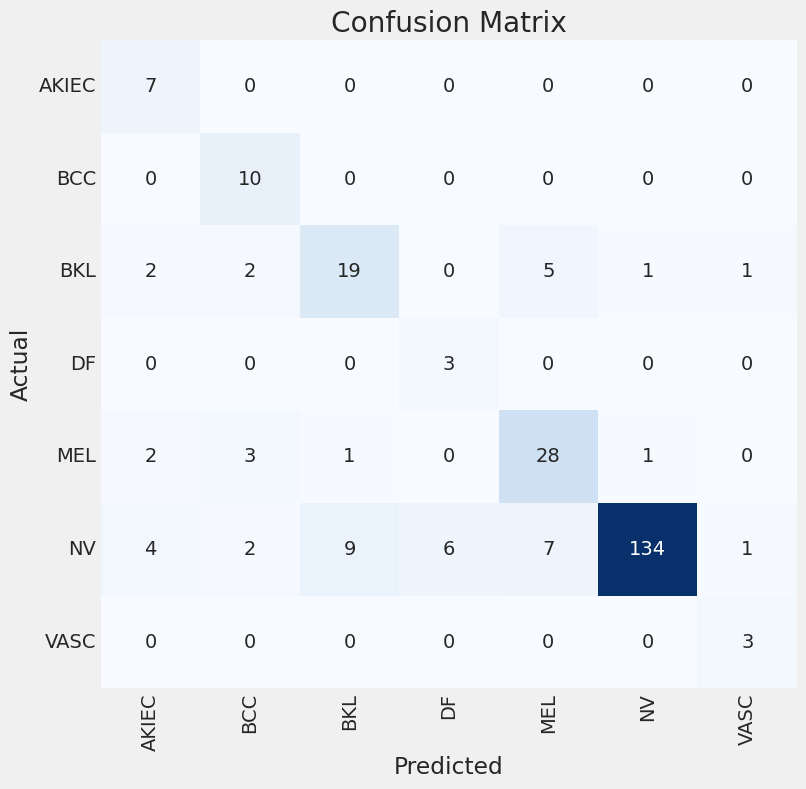
\includegraphics[width=0.8\textwidth]{./Graphics/confussionmatrix_p1.png}
   \caption{Estadísticas de eficacia del modelo al estimar los resultados en el conjunto de pruebas\label{fig:confussion_matrix_p1}}
   \end{center}
   \end{figure}

   \begin{figure}[ht]%
      \begin{center}
      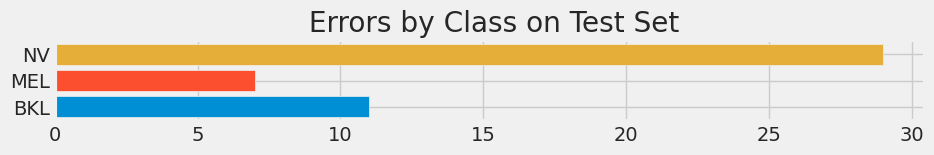
\includegraphics[width=0.8\textwidth]{./Graphics/errorByClass_p1.png}
      \caption{Gráfico de errores por clase en el conjunto de pruebas\label{fig:class_errors_p1}}
      \end{center}
      \end{figure} 


La matriz de confusión proporciona información valiosa sobre el rendimiento del modelo en relación de Actual/Predicho, en términos de su capacidad para clasificar correctamente cada una de las siete clases de cáncer de piel. La diagonal principal de la matriz representa los verdaderos positivos (TP), el número de casos en los que el modelo ha predicho correctamente la clase correspondiente. Los valores fuera de la diagonal principal indican errores de clasificación.

    La clase 'NV' muestra una alta cantidad de clasificaciones correctas (134), pero también tiene errores significativos al ser confundida con otras clases (como 'BKL' y 'MEL'). La clase 'AKIEC' resultó la más difícil de predecir, con la mayoría de las muestras mal clasificadas. Esto puede deberse a la similitud entre las características de estas clases, pero sobre todo al desbalance en el conjunto de datos.
    
    Cada barra representa el número de muestras de una clase particular que fueron mal clasificadas.

\subsection*{Informe de clasificación}

\begin{table}[ht]
    \centering
    \caption{Informe de clasificación para el Experimento 1}
    \label{tab:classification_report_exp1}
    \begin{tabular}{lcccc}
    \hline
    \textbf{Categoría Diagnóstica} & \textbf{Precisión} & \textbf{Recall} & \textbf{F1-Score} & \textbf{Soporte} \\
    \hline
    AKIEC & 0.47 & 1.00 & 0.64 & 7 \\
    BCC   & 0.59 & 1.00 & 0.74 & 10 \\
    BKL   & 0.66 & 0.63 & 0.64 & 30 \\
    DF    & 0.33 & 1.00 & 0.50 & 3 \\
    MEL   & 0.70 & 0.80 & 0.75 & 35 \\
    NV    & 0.99 & 0.82 & 0.90 & 163 \\
    VASC  & 0.60 & 1.00 & 0.75 & 3 \\
    \hline
    \textbf{Accuracy} & & & 0.81 & 251 \\
    \textbf{Macro Avg} & 0.62 & 0.89 & 0.70 & 251 \\
    \textbf{Weighted Avg} & 0.86 & 0.81 & 0.83 & 251 \\
    \hline
    \end{tabular}
    \end{table}

Resultados Generales: La precisión global del modelo fue del 81\%, con una media ponderada de precisión del 86\%, recall del 81\%, y una puntuación F1 del 83\%.
Resultados por Categoría Diagnóstica: Describir la precisión, el recall, y la puntuación F1 para cada categoría diagnóstica, destacando que 'NV' tuvo la precisión más alta (0.99) y 'AKIEC' la más baja (0.47). El recall fue perfecto (1.00) para 'AKIEC', 'BCC', 'DF', y 'VASC', lo que indica que todas las muestras verdaderas fueron identificadas correctamente, pero la precisión varió, sugiriendo un posible desequilibrio en la identificación de falsos positivos.

\section{Experimento 2: Análisis de la estratificación de datos en la clasificación de imágenes de cáncer de piel}

%-----------------------------------------------------------------------------------
\subsection*{Estadísticas básicas}\label{sub:basic_statistics_p2}
%-----------------------------------------------------------------------------------
    
    Estos resultados de la tabla siguiente corresponden a la evaluación del modelo a lo largo de 40 epochs (o iteraciones) de entrenamiento. Cada fila representa una época y se presentan las siguientes métricas:
    
    \begin{figure}[ht]
      \small
      \begin{center}
          \begin{tabular}{|c|c|c|c|c|c|c|c|} \hline
          E & Loss & Acc & V loss & V acc & LR & M & Batch \\ \hline
          1 & 9.587 & 40.581 & 8.95658 & 56.800 & $10^{-2}$ & accuracy & 85.25 \\ \hline
          2 & 7.798 & 67.615 & 7.67235 & 66.800 & $10^{-2}$ & accuracy & 21.72 \\ \hline
          3 & 6.884 & 79.340 & 6.96014 & 69.600 & $10^{-2}$ & accuracy & 22.56 \\ \hline
          4 & 6.214 & 87.365 & 6.35865 & 71.200 & $10^{-2}$ & accuracy & 25.81 \\ \hline
          5 & 5.646 & 91.690 & 5.94812 & 75.200 & $10^{-2}$ & val\_loss & 23.08 \\ \hline
          6 & 5.172 & 92.999 & 5.44954 & 76.800 & $10^{-2}$ & val\_loss & 23.23 \\ \hline
          7 & 4.735 & 94.479 & 5.06016 & 76.400 & $10^{-2}$ & val\_loss & 23.19 \\ \hline
          8 & 4.334 & 96.528 & 4.73837 & 76.800 & $10^{-2}$ & val\_loss & 22.90 \\ \hline
          9 & 3.969 & 97.211 & 4.33689 & 77.200 & $10^{-2}$ & val\_loss & 22.74 \\ \hline
          10 & 3.631 & 98.008 & 4.15826 & 74.000 & $10^{-2}$ & val\_loss & 22.56 \\ \hline
          11 & 3.315 & 98.406 & 3.89153 & 73.600 & $10^{-2}$ & val\_loss & 23.11 \\ \hline
          \dots & \dots & \dots & \dots & \dots & \dots & \dots & \dots \\ \hline
          34 & 0.627 & 99.886 & 1.24470 & 76.800 & 0.00013 & val\_loss & 23.30 \\ \hline
          \end{tabular}
          \caption{Estadísticas básicas de algunas iteraciones del modelo EfficientNetB1.}
      \end{center}\label{fig:estadisticas_p2}
  \end{figure}
    
    En general, los resultados muestran que el modelo mejora con el tiempo, ya que la pérdida disminuye y la precisión aumenta tanto en el conjunto de datos de entrenamiento como en el de validación.

%-----------------------------------------------------------------------------------
\subsection*{Estadísticas de aprendizaje}\label{sub:learning_statistics_p2}
%-----------------------------------------------------------------------------------
		\begin{figure}[ht]%
      \begin{center}
      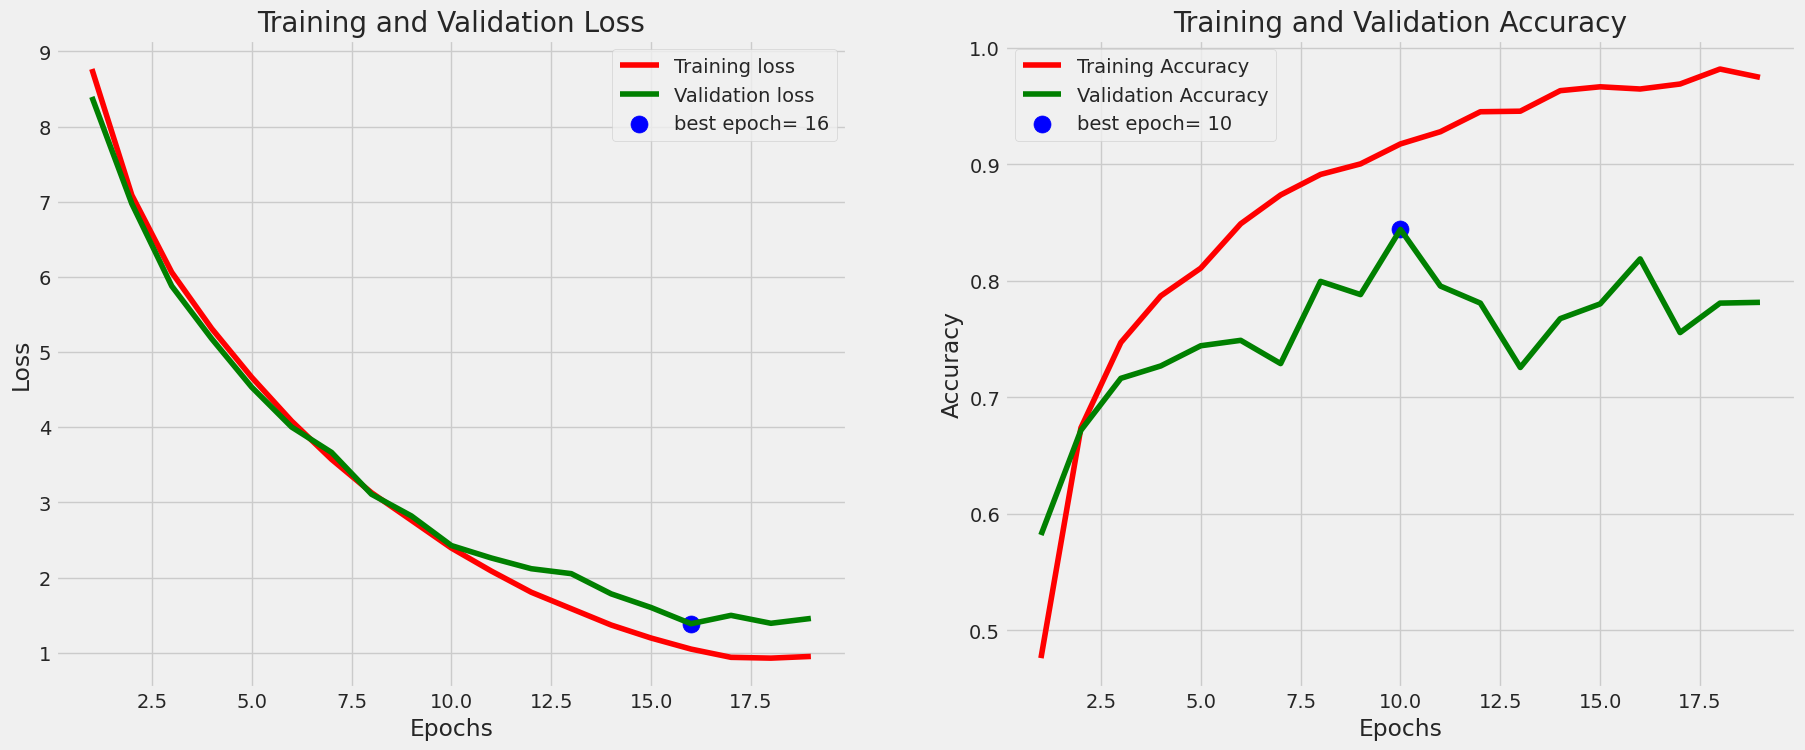
\includegraphics[width=1\textwidth]{./Graphics/training&validation_p2.png}
      \caption{Estadísticas de aprendizaje a lo largo del proceso de entrenamiento.\label{fig:training_validation_loss_p2}}
      \end{center}
		\end{figure}
  
La época con la mejor pérdida de validación y la mejor precisión de validación no coinciden, sugiere un trade-off entre la optimización de la pérdida y la maximización de la precisión. La volatilidad en la precisión de validación sugiere que el modelo puede beneficiarse de un ajuste en el tamaño del lote para suavizar las actualizaciones de los pesos y mejorar la estabilidad del modelo.

Dado lo anterior, se hizo una última iteración del modelo aumentando el volumen de muestras por clase a 500. Estos fueron los resultados. Se obtuvo una efectividad de aproximadamente 87\% (86.83\%).

\begin{figure}[ht]%
   \begin{center}
   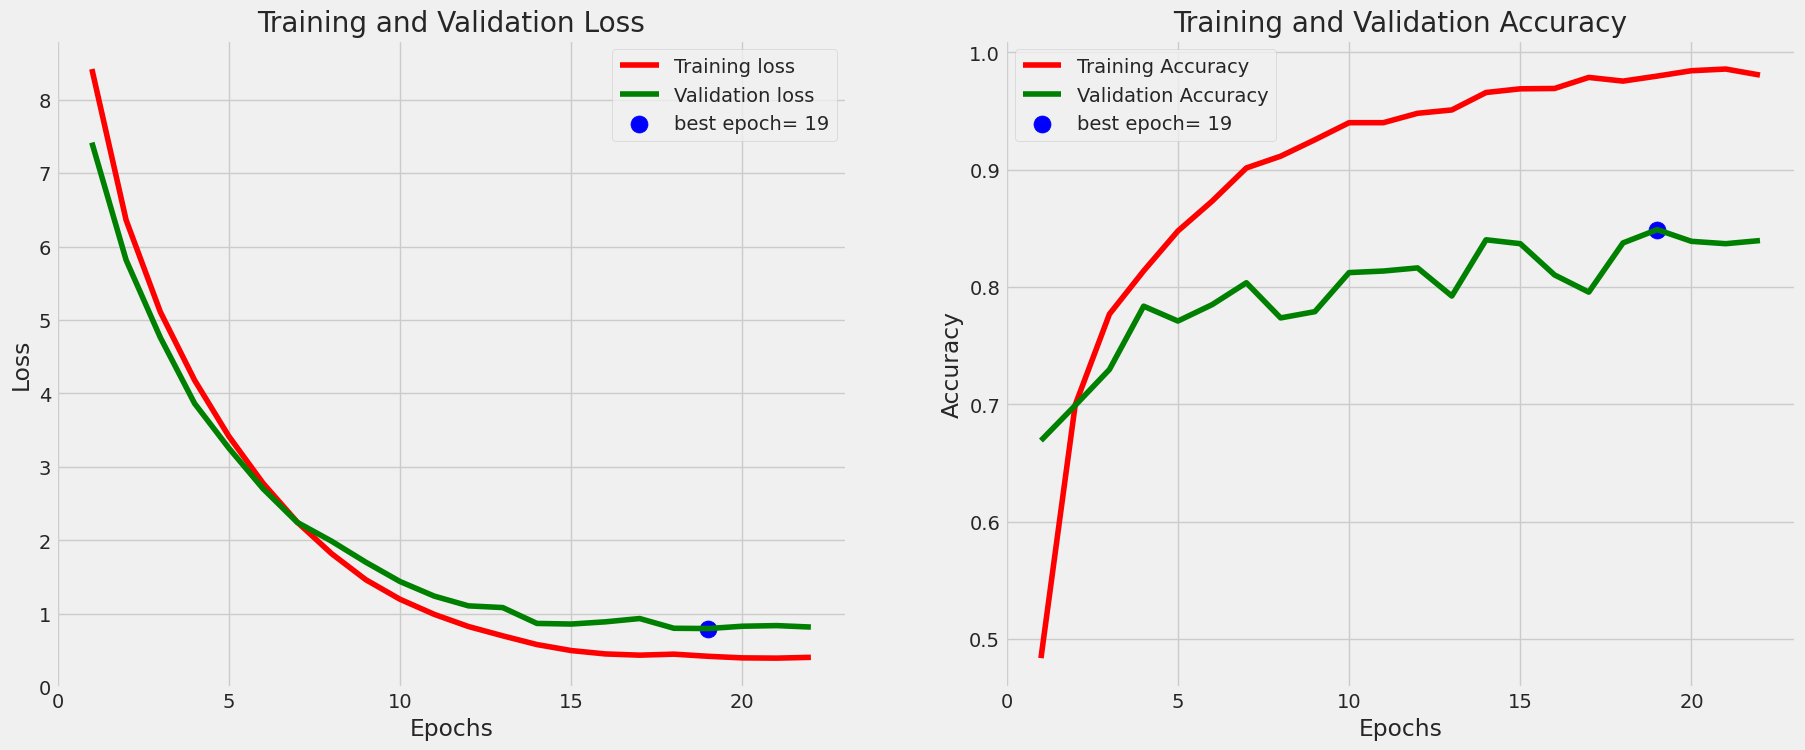
\includegraphics[width=1\textwidth]{./Graphics/training&validation_p3.png}
   \caption{Estadísticas de aprendizaje a lo largo del proceso de entrenamiento.\label{fig:training_validation_loss_p3}}
   \end{center}
   \end{figure}

La disminución continua en la pérdida de entrenamiento y la tendencia ascendente en la precisión de entrenamiento sugieren que el modelo está aprendiendo de manera efectiva y consistente. La pérdida de validación que converge con la de entrenamiento y la mejor época coincidente para pérdida y precisión de validación (época 19) indican que el modelo generaliza bien y no solo memoriza los datos de entrenamiento.

En el gráfico actual, hay una mejor alineación entre la pérdida de entrenamiento y validación y menos volatilidad en la precisión de validación, lo que indica un modelo más estable.

%-----------------------------------------------------------------------------------
\subsection*{Estadísticas de eficacia}\label{sub:accuracy_statistic_p2}
%-----------------------------------------------------------------------------------
    
\begin{figure}[ht]%
   \begin{center}
   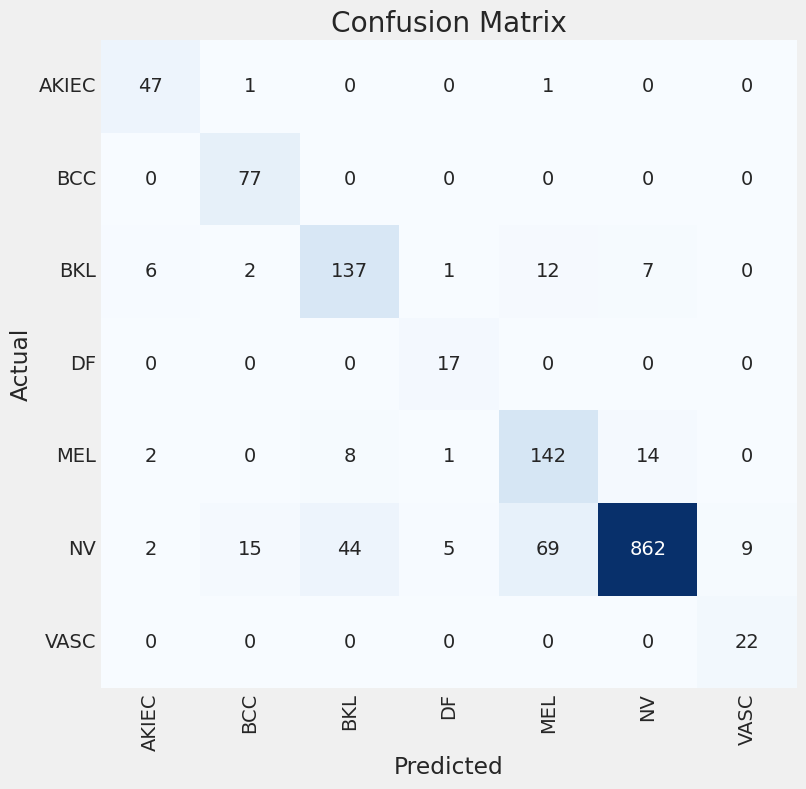
\includegraphics[width=0.8\textwidth]{./Graphics/confussionMatrix_p3.png}
   \caption{Estadísticas de eficacia del modelo al estimar los resultados en el conjunto de pruebas\label{fig:confussion_matrix_p3}}
   \end{center}
   \end{figure}

   \begin{figure}[ht]%
      \begin{center}
      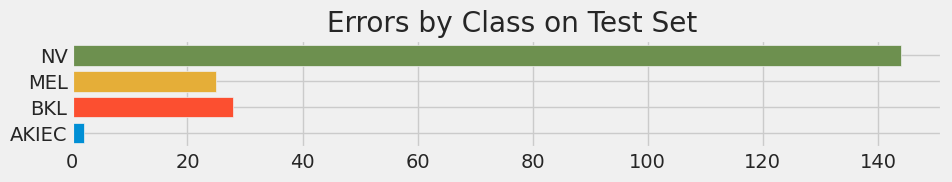
\includegraphics[width=0.8\textwidth]{./Graphics/errorByClass_p3.png}
      \caption{Gráfico de errores por clase en el conjunto de pruebas\label{fig:class_errors_p3}}
      \end{center}
      \end{figure}

NV muestra la mayoría de los errores, lo que puede deberse a una mayor prevalencia en el conjunto de datos.

Comparando ambos gráficos, podemos identificar áreas específicas donde el modelo necesita mejora. Por ejemplo, la clase 'NV', a pesar de tener muchas predicciones correctas, tiene un número relativamente alto de falsos positivos y falsos negativos, lo que sugiere que puede haber características de las imágenes 'NV' que se confunden con otras clases. En cambio, 'BCC' y 'DF' parecen estar bien diferenciados del resto. Esto puede informar estrategias futuras para mejorar la precisión del modelo, como la recolección de más datos o la implementación de técnicas de aprendizaje más avanzadas para clases específicas.

\subsection*{Informe de clasificación}

    
    \begin{table}[H]
        \centering
        \caption{Informe de clasificación para el Experimento 2}
        \label{tab:classification_report_exp2}
        \begin{tabular}{lcccc}
        \hline
        \textbf{Categoría Diagnóstica} & \textbf{Precisión} & \textbf{Recall} & \textbf{F1-Score} & \textbf{Soporte} \\
        \hline
        AKIEC & 0.82 & 0.96 & 0.89 & 49 \\
        BCC   & 0.81 & 1.00 & 0.90 & 77 \\
        BKL   & 0.72 & 0.83 & 0.77 & 165 \\
        DF    & 0.71 & 1.00 & 0.83 & 17 \\
        MEL   & 0.63 & 0.85 & 0.73 & 167 \\
        NV    & 0.98 & 0.86 & 0.91 & 1006 \\
        VASC  & 0.71 & 1.00 & 0.83 & 22 \\
        \hline
        \textbf{Accuracy} & & & 0.87 & 1503 \\
        \textbf{Macro Avg} & 0.77 & 0.93 & 0.84 & 1503 \\
        \textbf{Weighted Avg} & 0.89 & 0.87 & 0.87 & 1503 \\
        \hline
        \end{tabular}
        \end{table}
        
Resultados Generales: La precisión global del modelo fue del 87\%, con una media ponderada de precisión del 89\%, recall del 87\%, y una puntuación F1 del 87\%.
Resultados por Categoría Diagnóstica: Enumerar la precisión, el recall, y la puntuación F1 para cada categoría diagnóstica. Resalta que todas las categorías mejoraron en comparación con el Experimento 1, con 'NV' mostrando nuevamente la precisión más alta (0.98) y 'MEL' la más baja (0.63).



\section{Comparación entre los Experimentos}\label{subsubsec:comparison_exp}
%-----------------------------------------------------------------------------------

Eficiencia del Modelo: El Experimento 2 demuestra una eficiencia general superior con una mayor precisión de validación y un modelo más estable. Esto puede atribuirse a un balance más efectivo de clases y a ajustes en la tasa de aprendizaje.

Manejo de Desequilibrio de Clases: El Experimento 2 maneja mejor el desequilibrio de clases, lo que se refleja en una mejor diferenciación entre ciertas categorías diagnósticas.

Generalización: El Experimento 2 muestra una tendencia más estable en la pérdida de validación y en la precisión, sugiriendo una mejor capacidad para generalizar a nuevos datos.

Implicaciones para la Clasificación de Cáncer de Piel: Estos resultados resaltan la importancia de la estratificación de datos y del balance de clases en la clasificación de imágenes médicas, especialmente en contextos donde la variabilidad entre categorías es significativa.

\subsection{Comparación de Ventajas y Desventajas}

Ventajas del Experimento 1
\begin{enumerate}
    \item Sensibilidad: El modelo del Experimento 1 demostró una alta sensibilidad, con un recall perfecto en varias categorías, lo que es crucial en aplicaciones médicas para evitar falsos negativos.
    \item Eficiencia en Categorías Específicas: Ciertas categorías como 'NV' tuvieron una precisión extremadamente alta, lo que sugiere una eficiencia notable en la identificación de esta condición común.
\end{enumerate}

Desventajas del Experimento 1
\begin{enumerate}
    \item Balance de Precisión-Recall: Aunque el modelo tenía un alto recall en algunas categorías, la precisión era baja, lo que podría resultar en un número más alto de falsos positivos.
    \item Consistencia en el Rendimiento: La variabilidad en el rendimiento entre categorías puede indicar una necesidad de ajustar el modelo o los datos para mejorar la consistencia.
\end{enumerate}

Ventajas del Experimento 2
\begin{enumerate}
    \item Mejora en Precisión y F1-Score: El modelo del Experimento 2 mostró mejoras en la precisión y puntuación F1 en todas las categorías, indicando un equilibrio más sólido entre la precisión y el recall.
    \item Rendimiento General: Con una precisión global y una puntuación F1 más altas que el Experimento 1, este modelo demostró ser más robusto y equilibrado.
\end{enumerate}

Desventajas del Experimento 2
\begin{enumerate}
    \item Potencial Sobreajuste: A pesar de la mejora en los indicadores, un rendimiento demasiado alto en el conjunto de entrenamiento podría sugerir un sobreajuste, especialmente si no se replica en datos independientes.
\end{enumerate}

\section{Consideraciones Finales}\label{subsubsec:final_considerations}
%-----------------------------------------------------------------------------------

Los resultados obtenidos son prometedores y sugieren que los modelos de aprendizaje profundo tienen un potencial considerable para mejorar la precisión y la eficiencia del diagnóstico del cáncer de piel


\backmatter

\begin{conclusions}
    Los resultados obtenidos muestran una alta eficacia (79\% aproximadamente) que puede estar sujeta a futuras mejoras del modelo y del algoritmo. 
    En general, los modelos de detección de cáncer de piel pueden tener una precisión del 85\% al 95\% o superior, dependiendo de la complejidad del problema, la calidad de los datos y la selección del algoritmo utilizado. 
    Sin embargo, el 78\% es un porcentaje elevado para los algoritmos de aprendizaje automático, y con algunas mejoras en el modelo puede incrementarse. 
    También se desprende de este resultado la intención de convertir este proyecto en un producto a gran escala para ser utilizado, inicialmente, por los profesionales sanitarios de atención primaria, como prueba complementaria de alta efectividad a la hora de derivar a un paciente con una lesión cutánea al área de oncología. 
    Con la premisa de convertir los resultados obtenidos en un producto al servicio de la sociedad, el equipo investigador pretende seguir investigando y desarrollando una solución mejor.
\end{conclusions}

\begin{recomendations}
    \subsection*{Datos: procesamiento y estrategias de normalización}

\begin{enumerate}
    \item Enriquecimiento de Datos: Complementar el conjunto de datos con imágenes adicionales de fuentes confiables para mejorar la robustez del modelo.
    \item Aumentar la Diversidad de Datos: Utilizar técnicas de aumento de datos para generar variantes adicionales de las imágenes existentes, como rotaciones, zoom, o cambios en el brillo, para mejorar la capacidad del modelo de generalizar a partir de nuevos datos.
    \item Balance de Clases mediante Aumento: Para categorías con menos ejemplos, aplicar técnicas de aumento de datos de manera selectiva para equilibrar la distribución de clases y reducir el sesgo del modelo.
    \item Estratificación Mejorada: Asegurarse de que la estratificación de datos se aplique de manera que todas las particiones (entrenamiento, validación, prueba) tengan una distribución representativa de cada clase.
\end{enumerate}

\subsection*{Modelo: optimización y ajuste de hiperparámetros}

\begin{enumerate}
    \item Regularización y Arquitectura de Red: Explorar diferentes parámetros de regularización, para dropout y L1/L2 para encontrar el mejor equilibrio entre el rendimiento y la prevención del sobre-ajuste.
    \item Presición y sesgos: Implementar modelos más complejos de clasificación para las clases menos representadas.
    \item Optimizadores: Utilizar otros optimizadores como RMSprop o SGD para mejorar la velocidad de convergencia y el rendimiento del modelo.
\end{enumerate}

\end{recomendations}

\printbibliography[heading=bibintoc]


\end{document}